\label{chap:05_dataset_creation}

Por lo marcado en la discusión de la anterior sección, consideramos interesante el problema de analizar el impacto del contexto en la detección de lenguaje discriminatorio. Antes de proseguir, podemos preguntarnos: ¿a qué nos referimos con el término ``contexto''? La contextualización, según John Cook-Gumperz, es:

\begin{displayquote}[\citet{gumperz1992contextualization}]
    (el) uso que hacen hablantes y oyentes de señales verbales y no verbales para poder conectar lo que se dice en un momento con el conocimiento adquirido a través de la experiencia para poder mantener la participación en la conversación y entender lo que se pretende decir.
\end{displayquote}

En este sentido, cualquier señal que pueda ayudar a entender las intenciones del interlocutor en una red social es información que ayuda a situar los mensajes: desde el hilo de una conversación, la noticia a la que hace referencia, el historial de conversaciones previas entre los interactores, información sociocultural de los interlocutores, entre otras \cite{sheth2021defining}. Para poner un ejemplo de por qué es necesario disponer de información adicional al comentario analizado, el mensaje ``sos un hombre'' en solitario puede parecer inofensivo; ahora, si ese mismo mensaje está dirigido hacia una mujer trans, su sentido es claramente discriminatorio. El comentario --con claro tono agresivo-- ``hay que tirar una bomba ahí'' puede tener carácter discriminatorio si lo consideramos en el contexto de una nota que habla sobre China y el COVID-19; sin embargo, es distinto si estamos hablando de un partido de fútbol, donde el remitente de un club manifiesta su enemistad contra otro equipo.


Vimos en el anterior capítulo que muchos mensajes analizados no se entendían bien al carecer de información contextual, tanto conversacional o del tópico al que hace cuestión. En líneas generales, la mayoría de los problemas de NLP sobre textos sociales suelen plantearse sobre comentarios sin ningún otro tipo de dato de quién lo emite \todo{chequear tilde}, a quién se lo dirige, ni sobre qué tema está hablando. Para analizar esto desde el problema de la detección de discurso de odio, nos abocamos en primer lugar a la tarea de crear un conjunto de datos que no sólo contenga un mensaje/comentario, sino que provea un contexto para éste. Un ámbito natural para esta tarea son las notas periodísticas, donde disponemos de un artículo y comentarios realizados sobre la nota. En este escenario, el comentario es el texto a analizar, mientras que el contexto está dado por la nota.

Muchos sitios de noticias disponen de sistemas embebidos de comentarios, pero vista la dificultad para la recolección y los limitados datos provistos por estos sitios acerca de sus usuarios nos llevaron a buscar otro medio: Twitter. Esta red social provee una sencilla API para descargar datos, a la vez que tiene términos y condiciones amigables para poder publicarlos. Así mismo, podemos pensar que algunas secciones de Twitter operan de una manera similar a un foro de comentarios de un sitio de noticias. Este dominio (comentarios sobre artículos periodísticos) tiene una naturaleza particular ya que las agresiones discriminatorias son usualmente a personajes públicos o colectivos de personas, y se dan de manera indirecta (a través del comentario en la noticia) y no directa (es decir, como respuesta al usuario de Twitter ofendido).

El trabajo realizado en este capítulo tuvo lugar en el contexto de un Proyecto Interdisciplinario de la UBA\footnote{\url{https://cyt.rec.uba.ar/vinculacion-transferencia/piuba/}} junto a sociólogos, abogados, lingüistas, y computólogos. Particularmente, el trabajo de la construcción del manual de etiquetado fue discutido en conjunto, contemplando varias perspectivas a la hora de armar una definición propia (algunas de estas ya fueron vertidas en la discusión en la Sección \ref{sec:hate_speech_definitions}). Teniendo en cuenta que muchos trabajos del área de detección de discurso de odio mediante técnicas de NLP no se realizan desde una mirada interdisciplinaria, es un aspecto a remarcar de la construcción de este recurso.

\section{Trabajo previo}
\label{sec:dataset_previous}

Pocos trabajos del área de detección de lenguaje abusivo o discurso de odio incorporan algún tipo de contexto a los comentarios recolectados para estas tareas. En esta sección haremos una revisión de los trabajos que han abordado la construcción de recursos que contengan algún tipo de información contextual. \citet{gao-huang-2017-detecting} construyeron un conjunto de datos de lenguaje discriminatorio sobre 1518 comentarios del sitio de Fox News, siendo estos anotados por etiquetadores que observaron tanto el comentario como el titular de la noticia en conjunto. Sobre estos datos, los autores efectuaron experimentos de clasificación usando regresiones logísticas y redes neuronales. En estos experimentos, observaron que un clasificador (tanto lineal como neuronal) mejora su performance al consumir el título de la noticia, dando indicios de que se puede aprovechar el contexto para mejorar la detección de este fenómeno. Sin embargo, como marcan \citet{pavlopoulos2020toxicity}, este trabajo cuenta con algunos problemas: en primer lugar, el tamaño del dataset es pequeño, y está extraído de sólo 10 noticias, lo cual limita fuertemente los posibles contextos de los comentarios. A su vez, la anotación fue realizada mayormente por una única persona, lo cual hace poco confiables las etiquetas obtenidas. Finalmente, algunos detalles menores debieran ser analizados con mayor detalle, como por ejemplo la utilización de los nombres de usuarios como variables predictivas.

\citet{mubarak-etal-2017-abusive} recolectaron comentarios en árabe con contenido abusivo del portal Al Jazeera para distintos artículos periodísticos. Sin embargo, este dataset tiene un problema: los comentarios son presentados a los anotadores sobre noticias, ignorando todo el thread de la conversación. Esto hace que el contexto sea presentado de manera parcial.

Paralelamente a nuestro trabajo, \citet{pavlopoulos2020toxicity} analizaron el impacto de agregar contexto a la tarea de detección de toxicidad. En particular, plantearon dos preguntas:

\begin{itemize}
    \item ¿Qué tanto afecta el contexto a la toxicidad percibida por humanos en conversaciones online?
    \item ¿Puede el contexto ayudar a mejorar la performance de clasificadores de toxicidad en comentarios?
\end{itemize}

Para responder estos dos puntos, los autores construyeron dos datasets en base a Wikipedia Talk Pages \cite{hua-etal-2018-wikiconv}, un conjunto de datos de discusiones del sitio de Wikipedia. En primer lugar, armaron un pequeño conjunto de 250 comentarios anotados por dos grupos disjuntos de anotadores: uno de los grupos anotó los comentarios de manera contextualizada, viendo tanto el comentario en cuestión como el título de la discusión; el otro grupo sólo vio el comentario a anotar sin contexto alguno. En dicho experimento observaron que los anotadores que observaron el contexto percibieron 6.4\% de comentarios tóxicos versus un 4.4\% de quienes anotaron sin contexto, una diferencia significativa aplicando un test Mann-Whitney U. Desagregando estos resultados, observaron que 13 de los 250 comentarios (5.2\%) tuvieron diferencias de anotación entre los dos grupos, con 9 (3.6\%) comentarios donde aumentó la toxicidad percibida y 4 comentarios donde bajó la toxicidad al ser agregado el contexto.

Para responder la segunda pregunta, anotaron $20$ mil comentarios del mencionado foro, la mitad anotados por un grupo que etiquetó viendo el contexto y la otra que no lo vio. Entre todos los comentarios recolectados, eligieron aquellos con profundidad entre dos (respuestas directas) a cinco, y que fuesen entre 10 y 400 caracteres de largo. Luego, entrenaron varios clasificadores con técnicas del estado del arte, sobre los cuales pudieron observar que el contexto no pareciera mejorar significativamente la performance en la detección de toxicidad en comentarios. En el próximo capítulo nos extenderemos sobre las técnicas utilizadas por este trabajo.

\citet{xenos-2021-context} continuaron el trabajo de \citet{pavlopoulos2020toxicity} desagregando el resultado de la segunda pregunta. Puntualmente, y observando que sólo un porcentaje pequeño de los comentarios parecen ser incididos por el contexto en el trabajo anterior, construyeron una nueva tarea: estimación de sensibilidad al contexto. Para ello, y usando como base el conjunto de datos de Civil Comments \cite{borkan2019civil}, reanotan un subconjunto de sus comentarios usando información de contexto a través de crowdsourcing, y usando etiquetas de toxicidad en un estilo similar a una regresión ordinal: no tóxico, incierto, tóxico, y muy tóxico. Sobre las anotaciones originales (que fueron hechas sin contexto) y las nuevas anotaciones, definieron para cada comentario una sensibilidad al contexto, dada por:

\begin{equation}
    \delta(p) = s^{oc}(p) - s^{ic}(p)
\end{equation}

\noindent donde $s^{oc}$ es la fracción de anotadores sin contexto que marcaron toxicidad, y $s^{ic}$ los que no tienen contexto. En el siguiente capítulo haremos un repaso de los experimentos de clasificación obtenidos en este trabajo.

\citet{sheth2021defining}, en un trabajo muy reciente, señalaron algunas oportunidades y desafíos para incorporar fuentes de información más ricas a la tarea de detección de toxicidad. Por ejemplo, incorporar información como el background socio-cultural de los interactores puede ayudar a distinguir algunos tipos de reapropiación de términos potencialmente catalogados como tóxicos -- por ejemplo, personas afroamericanas interpelándose con términos racistas entre sí. Así mismo, el historial de interacción entre los usuarios puede ayudar a distinguir interacciones abusivas de charlas amistosas entre amigos que usan vocabulario potencialmente tóxico. Finalmente, se promueve el uso de contenido externo para acercarse lo más posible al conocimiento humano a través de conocimiento del contenido, el individuo (atacado) y la comunidad. Para ello, se promueve el uso de bases de conocimiento y knowledge-infusion learning \cite{gaur2020infusion} para combinar cómputo neuronal sobre datos no estructurados y estructurados.



\citet{wiegand2021implicitly} mencionan formas implícitas de abuso, mucho más complejas que las basadas solamente en palabras ofensivas. Por ejemplo, deshumanizaciones (``los judíos son una plaga que merece ser eliminada''), llamadas a la acción (``hay que tirar una bomba en ese país''), acusaciones (``los chinos inventaron el coronavirus''), entre otros tipos sutiles de comportamiento tóxico. También menciona que la mayoría de los datasets no consiguen capturar estos fenómenos debido a la forma de recolección usualmente basada en keywords.

\citet{sap2020social} plantean un esquema bastante más complejo dentro de la detección de toxicidad o lenguaje abusivo. El conjunto de datos presentado en ese trabajo consta de comentarios recolectados de diversas redes sociales que son analizados con un formalismo al que denominan \emph{Social Bias Frames}. Cada instancia está etiquetada jerárquicamente de acuerdo a: toxicidad, intencionalidad, obscenidad, si está dirigido a un grupo, a qué grupo, qué implicancia tiene (\emph{``los XXX son todos YYY''}), y si el emisor es perteneciente al mismo grupo social que está siendo en teoría atacado.

\section{Esquema del conjunto de datos}


%%
%%
%% Link a Draw
%% https://docs.google.com/drawings/d/1IcBITgNJN-tehmvnZqcSF9cUuWIpNKJg6yHI5yjNF9c/edit
%%
%%

\begin{figure}[t]
    \centering
    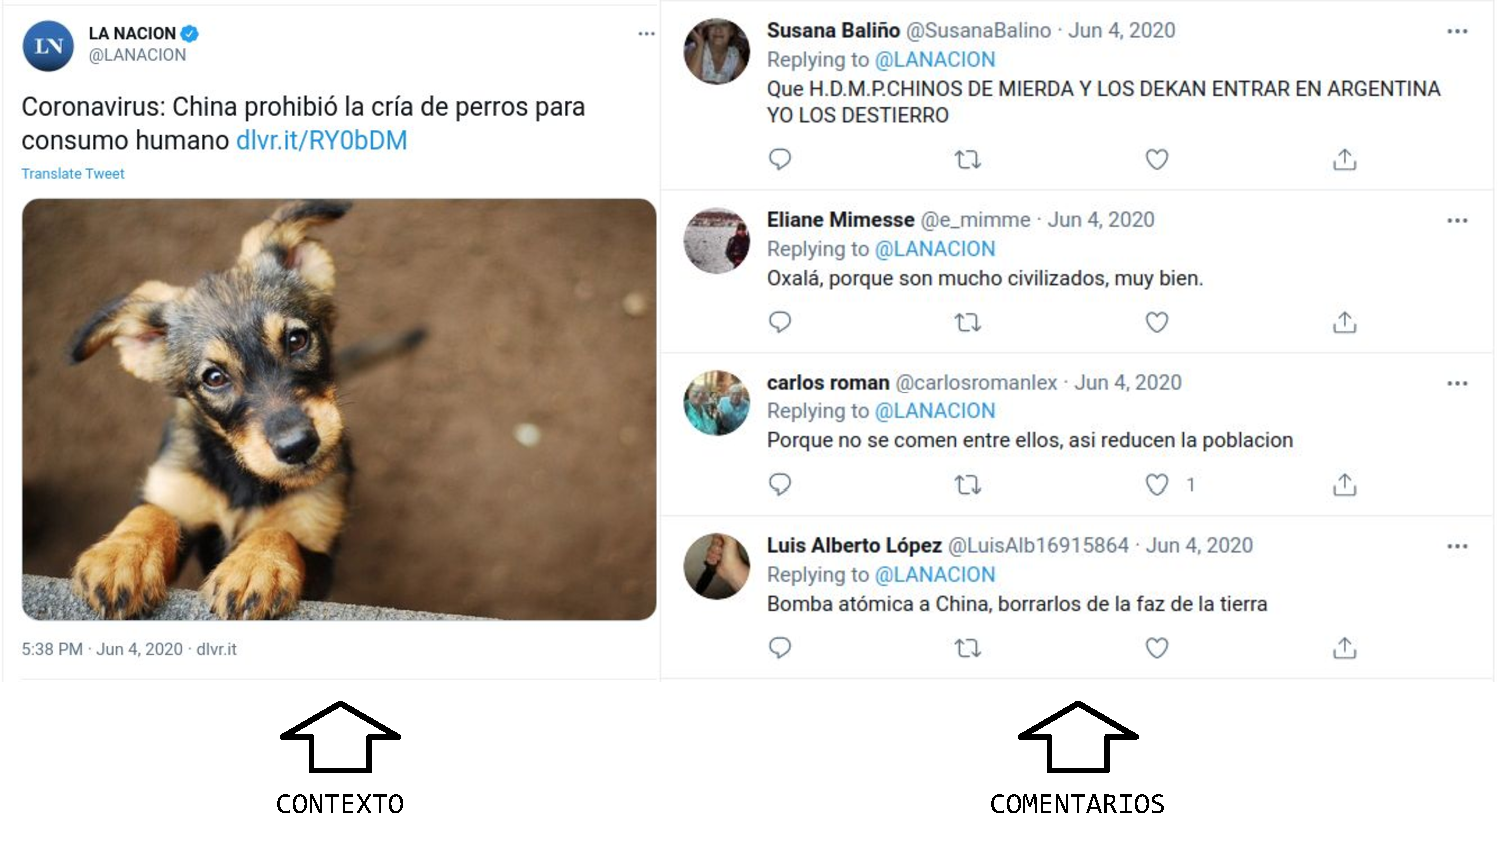
\includegraphics[width=\textwidth]{img/idea_dataset.pdf}
    \caption{Boceto del conjunto de datos: artículos periodísticos y sus respectivos comentarios en Twitter}
    \label{fig:idea_dataset}
\end{figure}

Para construir un conjunto de datos contextualizado analizamos algunas alternativas. Como vimos en otros trabajos, se puede entender el contexto de un mensaje de varias maneras: un contexto temático, donde sabemos que cierto comentario habla sobre un tema en particular; y un contexto conversacional, donde tenemos una secuencia de comentarios (un hilo o thread) y podemos extraer un comentario padre para cada uno salvo el raíz. La primera opción es la explorada por \citet{gao-huang-2017-detecting,mubarak-etal-2017-abusive}, donde recolectan comentarios de Fox News y Al-Jazeera respectivamente. El contexto conversacional, como hemos relatado anteriormente, es explorado en \citet{pavlopoulos2020toxicity} y \citet{xenos-2021-context}; sin embargo, como es marcado en el primer trabajo, la recolección de datos es no trivial, aún en un caso más amplio como el lenguaje abusivo, ya que la incidencia de comentarios de esta índole es relativamente baja. Es esperable que la tasa de ocurrencia de contenido discriminatorio sea aún menor, dificultando la recolección de datos interesantes para nuestro estudio.

Para analizar el impacto del contexto en la tarea de detección de discurso de odio, decidimos entonces ir por la primera opción: comentarios sobre notas periodísticas. No vamos a considerar un hilo de respuestas (contexto conversacional) sino simplemente aquellos comentarios que sean directos sobre el artículo periodístico. En ese punto, la idea sería similar a la de \citet{gao-huang-2017-detecting}, aunque una diferencia respecto a este conjunto de datos es la de incorporar dos modos de contexto: uno corto, donde sólo tengamos el título de la noticia; y uno largo, donde tengamos el texto completo del artículo.

Algo no menor a la hora de considerar la construcción del dataset es la posibilidad de publicar los datos. Por citar un ejemplo, el conjunto de datos recolectado por \citet{gao-huang-2017-detecting} es de libre acceso \footnote{\url{https://github.com/sjtuprog/fox-news-comments}} pero no queda claro que los términos y condiciones de la fuente permita esto. Más aún, si hubiésemos querido extraerlo de múltiples fuentes (por ejemplo, varios diarios), deberíamos chequear y/o acceder a permisos para cada sitio, a la vez que tendríamos el problema de tener fuentes diversas de los datos: diferentes longitudes, formatos, metadatos, entre otros.

Para evitar muchos de estos inconvenientes y poder reutilizar parte del trabajo desarrollado en esta tesis, decidimos recolectar comentarios en Twitter. Concretamente, decidimos recolectar respuestas de usuarios a posteos hechos por cuentas de medios. De alguna manera, esto emula un foro de comentarios de medios, teniendo la ventaja de un formato único para comentarios y un acceso a una audiencia de usuarios mucho más amplia que la de los microforos de cada sitio de noticias. La Figura \ref{fig:idea_dataset} ilustra un boceto de lo que queremos recolectar. A su vez, una ventaja de Twitter es que posee términos y condiciones de Twitter amigables para publicar los datos con fines de investigación. Las notas periodísticas fueron también descargadas pero debido a restricciones no tenemos aún en claro si podrán ser publicadas.

Finalmente, la elección del idioma. El conjunto de datos construido consta de comentarios realizados en idioma español, más precisamente en la variedad dialectal del Río de la Plata (español rioplatense). Una primera consideración al respecto de esto es la de generar recursos por fuera del inglés, un eje planteado para esta tesis. Por otro lado, también es importante señalar que el discurso de odio es un fenómeno cultural, y es importante que quienes estén a cargo de la construcción de este recurso sean conscientes del trasfondo sociolingüístico donde están situados los discursos discriminatorios. Es por eso que a lo largo de este capítulo tuvimos particular cuidado en esta dimensión, tanto desde el proceso de recolección hasta la selección de los anotadores que estén inmersos en la realidad cultural local.


\section{Proceso de construcción}

Dividiremos la construcción del dataset en tres etapas:

\begin{enumerate}
    \item Recolección: Proceso de recolección de datos de Twitter y de los artículos periodísticos
    \item Selección: Proceso de selección del conjunto de artículos y comentarios recolectados a etiquetar
    \item Anotación: Proceso de etiquetado de los artículos seleccionados
\end{enumerate}

Si bien en muchos casos las dos primeras etapas suelen ser la misma o bien la selección se limita a una muestra aleatoria de la recolección, este procedimiento sería muy ineficiente para nuestro estudio. Esto se debe a que en el dominio de comentarios periodísticos y discurso de odio, encontramos este tipo de discurso distribuido de manera muy poco uniforme, usualmente concentrado alrededor de ciertos tópicos disparadores. Para poder recolectar datos con una proporción razonable del fenómeno estudiado, evaluamos algunas posibilidades de selección de los artículos y sus respectivos comentarios.

En algunos trabajos previos, la recolección y selección constan conjuntamente de la búsqueda en base a ciertas palabras clave, que son utilizadas para recolectar tweets o bien para preseleccionar usuarios productores de discurso de odio \cite{waseem2016hateful,hateval2019semeval}. En nuestro caso, la selección de artículos y comentarios presenta cierta novedad y complejidad, con lo cual separamos este procedimiento para explicarlo detalladamente en las siguientes secciones.

% COLECCIÓN


\section{Recolección de datos}

En esta sección describiremos el proceso de recolección de datos. La salida de esta etapa será un conjunto de artículos y sus comentarios extraídos de Twitter. Describiremos a continuación las decisiones realizadas respecto a las fuentes y a decisiones técnicas realizadas.

\subsection{Diarios elegidos}

Limitamos nuestra recolección de datos a cuentas de diarios de la República Argentina y, puntualmente, nos centramos en diarios con comunidad mayormente rioplatense ya que (como comentaremos más adelante) los anotadores son nativos de esa variedad dialectal. Esto es teniendo en cuenta que esta tarea depende fuertemente de la jerga y de las variaciones dialectales de cada país decidimos realizar sólo anotación de estos diarios.

Además, si bien buscamos otros medios del interior (como por ejemplo ``La voz del Interior'', diario dirigido mayormente a un público fuera de la Metrópolis de Buenos Aires) observamos que la interacción en Twitter de estos medios es muy baja: pocos usuarios comentan sus notas. En pos de maximizar

Los diarios seleccionados fueron los siguientes:

\begin{itemize}
    \item @infobae
    \item @clarincom
    \item @perfilcom
    \item @LANACION
    \item @cronica
\end{itemize}


Si bien recolectamos notas de otros medios, no los consideraremos a partir de ahora, y los dejamos para análisis posteriores. Los medios elegidos son medios formales y tradicionales, la mayoría de ellos con soporte escrito. Consideramos la posibilidad de elegir medios no tradicionales y más orientados a grupos de la derecha ``alternativa'' (puntualmente, ``La Derecha Diario''\footnote{\url{http://twitter.com/laderechadiario}}). Estos medios son altamente generadores de contenido de odio. Sin embargo, finalmente tomamos la decisión de descartarlos de las subsiguientes etapas.


\subsection{Método de recolección}



La API de Twitter\footnote{Usamos la versión 1.1 de la API. La versión 2.0 parece facilitar la recopilación de conversaciones} en su versión gratuita, nos brinda dos modos de recolectar tweets de su plataforma:

\begin{enumerate}
    \item Search API: permite buscar tweets en base a términos, de hasta 15 días atrás sobre una pequeña muestra, recreando lo que vemos en la UI de Twitter
    \item Stream API: permite buscar tweets en tiempo real sobre una muestra de cerca del 1\% de todos los tweets de la red social
\end{enumerate}

La API Stream, mientras por un lado limita temporalmente la recolección de datos, por el otro nos brinda la posibilidad de recolectar una mayor cantidad de información en tiempo real. Más aún, dada la naturaleza de nuestros datos (discurso de odio), se corre el riesgo de que con el tiempo sean moderados e inaccesibles para cualquier búsqueda con la API Search. \todo{Mencionar algo de los términos y condiciones de Twitter}


Por lo explicado, usamos la API de Twitter Stream mencionando cualquiera de estas cuentas. Si estamos entonces recolectando tweets sobre \verb|@medio|, el proceso de recolección nos da:

\begin{enumerate}
    \item Tweets de \verb|@medio|
    \item Respuestas a los tweets de \verb|@medio|
    \item Tweets de terceros que mencionan a \verb|@medio|
    \item Retweets (RT) de tweets de \verb|@medio|
    \item Citas de tweets de \verb|@medio|
\end{enumerate}

Los RTs y tweets que arroben a \verb|@medio| carecen de interés para nuestro estudio, con lo cual los descartamos. Por otro lado, también descartamos las citas, aunque podrían entenderse como ``respuestas'' a los tweets originales. Nos quedamos con tweets de \verb|@medio| y las respuestas a estos. Si bien la API nos da estos tweets desestructuradamente, reconstruimos el árbol de la discusión mediante el campo \verb|in_reply_to_status_id|\footnote{Ver la documentación y la referencia al campo en \url{https://developer.twitter.com/en/docs/twitter-api/v1/data-dictionary/object-model/tweet}}.

Para el propósito de este trabajo, solo estamos interesados en el primer nivel de respuestas al tweet original, y no incorporaremos hilos de respuestas.

También eliminamos las URLs de los artículos de los enlaces.




\begin{table*}[t]
    \centering
    \begin{tabular}{ c|c|c }
        coronavirus  &  encierro          & síntomas \\
        covid        &  fase              & fiebre   \\
        cuarentena   &  infectados        & distanciamiento     \\
        normalidad   &  Wuhan             & aislamiento\\
    \end{tabular}
    \caption{Palabras usadas para recolectar artículos relacionados a COVID-19.\label{tab:article_words}}
\end{table*}


Accidentalmente, la recolección de datos se dio al mismo tiempo del estallido de la pandemia del COVID-19. Por ese motivo, y dadas las implicancias de la pandemia sobre el discurso discriminatorio en las redes sociales, se hizo foco en artículos relacionados con COVID-19. Para ello, seleccionamos artículos buscando una cantidad de palabras en su cuerpo, por lo que seleccionamos específicamente artículos relacionados con COVID-19. La tabla \ref{tab:article_words} contiene las palabras utilizadas para recuperar estos artículos.

\subsection{Datos recolectados}

\begin{table}[t]
    \centering
    \begin{tabular}{l|c|c}
    Medio      & \#Artículos & \#Comentarios \\
    \hline
    @infobae   &  45,652   &  822,462 \\
    @clarincom &  29,050   &  672,401 \\
    @perfilcom &  8,764    &  61,203  \\
    @LANACION  &  16,040   &  506,091 \\
    @cronica   &  17,250   &  70,872 \\
    \hline
    Total      & 116,756  & 2,133,029 \\
    \end{tabular}
    \caption{Artículos recoletados por medio}
    \label{tab:articulos_recoletados_por_medio}
\end{table}


En la tabla \ref{tab:articulos_recoletados_por_medio} damos los números de los artículos recolectados por cada medio, luego de aplicado. Si bien recolectamos más artículos de otros medios, no son enumerados. Infobae es el medio que más producción de artículos genera, y también será finalmente sobre el que más comentarios etiquetemos.

La figura \ref{fig:fecha_articulos_por_medio_todas} muestra la distribución temporal de los artículos, sin aplicar ningún filtro por palabras, mientras que \ref{fig:fecha_articulos_por_medio_covid} muestra aquellas relacionadas al COVID-19 utilizando el filtro de palabras listado en la tabla \ref{tab:article_words}. Podemos observar dos caídas. Hay un pequeño pozo en mayo 2020 que se debió a la caída de nuestros servidores de recolección. Por otro lado, observamos que algunos medios (particularmente La Nación) parecieran mencionar menos directamente al COVID (al menos con los términos referidos anteriormente) hasta un nuevo pico cerca de fin de año, coincidente con un nuevo rebrote del virus en este país.

Sin embargo, todo esto puede ser un artefacto del método de filtrado: muchas notas contienen links a otras con sus títulos y eso puede interferir en estas estimaciones. Así y todo, decidimos mantener este método ya que consideramos que mayormente las notas en el período referido tienen relación con la pandemia.

Si bien en las siguientes secciones realizaremos un filtrado de la mayoría de estos artículos previamente a la anotación, utilizaremos este conjunto de datos no supervisado para efectuar ajustes de dominio en la siguiente sección.

\begin{figure}
    \centering
    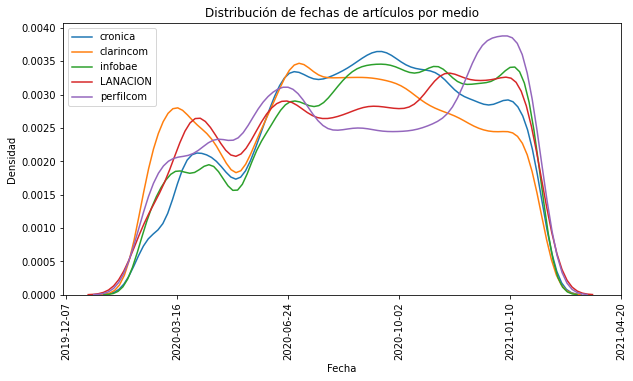
\includegraphics[width=\textwidth]{img/fechas_por_medios_todas.png}
    \caption{Distribución temporal de artículos recolectados}
    \label{fig:fecha_articulos_por_medio_todas}
    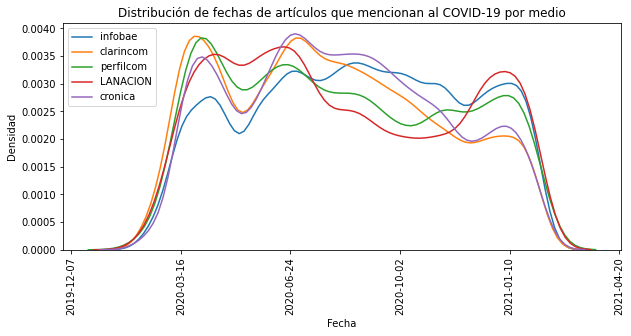
\includegraphics[width=\textwidth]{img/fechas_por_medios.png}
    \caption{Distribución temporal de artículos recolectados que mencionan COVID-19 o algún término relacionado}
    \label{fig:fecha_articulos_por_medio_covid}
\end{figure}


% SELECCIÓN
\section{Selección de datos a anotar}


Un problema que se presenta antes de comenzar el etiquetado es el de seleccionar los artículos que vamos a etiquetar, teniendo en consideración la gran cantidad de datos recolectados y los recursos disponibles. Una primera posibilidad para esto es realizar una selección aleatoria de artículos y comentarios. Sin embargo, los comentarios discriminatorios no se distribuyen de manera uniforme entre los artículos sino que se concentran sobre algunos temas que generan este tipo de contenido. Es mucho más probable encontrar comentarios de índole discriminatoria en notas que tengan temas cercanos a alguna de las características protegidas: por ejemplo, es esperable que encontremos contenido discriminatorio en notas sobre China y el Coronavirus o sobre una chica transgénero antes que en un artículo de fútbol o economía. Si bien una selección aleatoria preservaría una tasa de incidencia mucho más cercana a la observada en el universo de comentarios, es más importante poder obtener una mayor cantidad de observaciones que reflejen el fenómeno estudiado.

Teniendo esto en cuenta, evaluamos varias alternativas para realizar la selección de artículos. La primera fue intentar seleccionar aquellos artículos que consideramos como candidatos a fomentar contenido discriminatorio. Una posibilidad para esto sería usar algunas palabras semilla para seleccionar artículos interesantes en base a ciertos temas que consideramos relevantes.

Otra posibilidad evaluada fue la de buscar directamente comentarios que marquen que ese artículo suscita contenido discriminatorio. Para ello, podemos listar algunos insultos comunes o expresiones peyorativas hacia los grupos protegidos considerados. Es necesario remarcar que esto lo hacemos para seleccionar \tbf{artículos} y no los comentarios que contengan esos insultos; hacer esto último nos genera una muestra muy distorsionada y tendiente a encontrar el fenómeno más explícito de la discriminación (el insulto racista, homofóbico, etc.). Esta estrategia guarda relación con la descripta por \citet{hateval2019semeval} para seleccionar usuarios generadores de contenido discriminatorio.

Describimos a continuación las alternativas analizadas para seleccionar los artículos y sus respectivos comentarios.


\subsection{Selección en base a artículos}

\begin{table}[b!]
    \centering
    \small
    \begin{tabular}{p{0.21\textwidth}  p{0.26\textwidth} p{0.23\textwidth} p{0.19\textwidth}}
    \hline
    China        &  piqueteros              &  mamá                & domésticas            \\
    Cuba         &  villas                  &  de género           & la modelo             \\
    cubano       &  la villa                &  aborto              & la periodista         \\
    bolivia      &  movimientos sociales    &  actriz              & la cantante           \\
    paraguayo    &  organizaciones sociales &  actrices            & travesti              \\
    judío        &  tomas de tierras        &  feminista           & trans                 \\
    camionero    &  toma de tierras         &  femicidio           & gay                   \\
    ladrón       &  sindicatos              &  enfermera           & homosexual            \\
    represión    &  Guernica                &  madre               & de la V               \\
    criminal     &  mapuches                &  Ofelia              &                       \\
    \hline
    \end{tabular}
    \caption{Palabras semilla utilizadas para la selección de artículos. Cada palabra se busca sobre el cuerpo del artículo candidato a ser etiquetado}
    \label{tab:palabras_articulos}
\end{table}

En primer lugar, consideramos la posibilidad de hacer una selección en base al contenido de los artículos. Luego de hacer un análisis exploratorio de los datos usando LDA \cite{blei2003latent} para buscar tópicos posibles de las notas, decidimos realizar una selección controlada y determinística en base a la utilización de palabras y expresiones clave. Estas expresiones las recolectamos de manera subjetiva y en base a la observación de los tópicos y de nuestra percepción de la generación de discurso discriminatorio en los comentarios de los usuarios.

La Tabla \ref{tab:palabras_articulos} muestra el conjunto de expresiones utilizado para recolectar artículos. Como vemos, hay diversas palabras que recogen temáticas de posibles tópicos generadores de contenido discriminatorio, algunos muy locales respecto a eventos concretos durante la pandemia. Si algún artículo contiene una de las expresiones mencionadas, es seleccionado para ser etiquetado.

Para realizar esta búsqueda de términos en el cuerpo de los artículos, indexamos los textos en \emph{MongoDB}\footnote{\url{https://www.mongodb.com/}}, una base de datos no relacional. Este motor de bases de datos permite la utilización de índices en base a texto, permitiendo realizar búsquedas en base a expresiones, palabras, e inflexiones.



\subsection{Selección en base a comentarios}
\label{subsec:seleccion_comentarios}


\begin{table*}[h]
    \centering
    \small
    \begin{tabular}{l l l l l l l}
    \hline
    bija          & urraca     & viejo puto    & trolo      & peruano  & matarlos         & negra      \\
    prostituta    & tucán      & trabuco       & sodomita   & peruca   & una bomba        & negro de   \\
    feministas    & putita     & travesti      & chinos de  & judío    & vayan a laburar  & negros     \\
    feminazis     & reventada  & trava         & bolita     & sionista & vayan a trabajar & bala       \\
    aborteras     & marica     & degenerado    & paraguayo  & villeros & gorda            & uno menos  \\
    \hline
    \end{tabular}
    \caption{Palabras utilizadas para recolectar comentarios}
    \label{tab:palabras_comentarios}
\end{table*}

Otra posibilidad para seleccionar artículos candidatos a ser etiquetados es la de observar los comentarios de usuarios en lugar del texto completo de éste. En base a los comentarios, podemos tener alguna medida de si el artículo suscita reacciones potencialmente discriminatorias. Por ejemplo, si observamos que en un artículo hay comentaristas que usan expresiones discriminatorias contra la comunidad LGBTI, podemos pensar que el contenido de la noticia es interesante para nuestro estudio.

El procedimiento para este tipo de selección es similar al mencionado anteriormente con artículos, sólo que aplicado a comentarios: buscamos respuestas de usuarios que contengan alguna de las expresiones semilla listadas en la Tabla \ref{tab:palabras_comentarios}. Estas palabras fueron recolectadas de manera subjetiva en base a la observación y a la experimentación sobre los datos, tratando de contener diversas expresiones de contenido mayormente discriminatorio. La lista contiene expresiones ofensivas para diversas características de interés: insultos racistas, homofóbicos, misóginos; insultos dirigidos dirigidos a algún personaje particularmente atacado en las redes sociales; expresiones de odio de clase; etc.

Dado un artículo, marcamos los comentarios que contengan una o más de las expresiones listadas. Si el artículo tiene tres o más comentarios marcados, entonces el artículo es seleccionado; caso contrario, es descartado. Vale remarcar que este proceso de selección es para los \emph{artículos}, no para los comentarios. De lo contrario, sólo buscaríamos respuestas que contengan alguna de estas expresiones.

Luego de algunos análisis experimentales y observacionales de las dos posibles metodologías, decidimos utilizar el muestreo de artículos en base a comentarios. En base a un análisis subjetivo, los artículos seleccionados parecían tener mayor incidencia de mensajes discriminatorios y eso nos decantó hacia esa opción.

Una posibilidad adicional analizado fue utilizar un clasificador que nos señale posibles comentarios discriminatorios, usando esta información para seleccionar artículos candidatos a etiquetar. Para ello, aplicamos un clasificador basado en BETO \cite{canete2020spanish} entrenado sobre el dataset de \hateval{} (ver sección \ref{chap:04_hate_speech}) sobre los comentarios de los artículos. Una evaluación subjetiva de esto nos dio pobres resultados, tanto porque no captaba algunas agresiones discriminatorias (de características no incluídas en el dataset de \citet{hateval2019semeval}) como muchos falsos positivos o errores debido al cambio de dominio (temático y también dialectal). Si bien descartamos este método, puede ser de relevancia usar algún método que no esté basado en palabras semillas o utilizar algún método semi-automático para encontrar candidatos a etiquetar.


\subsection{Muestreo de comentarios}

Una vez que seleccionamos los artículos, resta decidir qué comentarios vamos a anotar. No podemos seleccionar todos ya que muchos artículos cuentan con una cantidad importante de comentarios (en el orden de los cientos) y es deseable mantener un balance entre los comentarios anotados por artículo. Tampoco es deseable (en pos de maximizar el producto de la anotación) seleccionar comentarios de artículos escasamente discutidos. Teniendo esto en mente, conservamos sólo los comentarios de artículos que tengan al menos 20 comentarios. Luego, para cada artículo, seleccionamos aleatoriamente hasta 50 comentarios entre aquellos que no contengan URLs u otro contenido no textual.

En este punto, consideramos el muestreo aleatorio como la forma menos sesgada para seleccionar nuestros comentarios, pero mencionamos de todas formas algunas alternativas evaluadas. Una fue la de considerar todo el universo de comentarios y seleccionar la muestra de allí. Sin embargo, esto sobrerrepresentaría a aquellos temas muy comentados, siendo muchos de ellos acerca de temas políticos que se filtraron en nuestra selección. Otra consideración posible es la de utilizar información de usuarios y sus conexiones, información que Twitter nos brinda a través de los followers de cada usuario. Muchos usuarios que generan contenido discriminatorio en redes sociales se agrupan en comunidades: subgrafos de usuarios altamente conectados entre sí. Usar algún tipo de información sobre esto (por ejemplo, con algún algoritmo como el de Louvain \cite{blondel2008fast}) podría auxiliar al balance de comentarios posiblemente discriminatorios. Para un ejemplo de la utilización de esta técnica, \citet{lai2018stance} y \citet{furman2021you} usan este tipo de algoritmos como manera semi-supervisada de detectar las posturas de los usuarios respecto a distintos temas.


% ANOTACIÓN
\section{Anotación}

Hasta este momento describimos la recolección de los datos, a lo cual le siguió la selección de los artículos y comentarios a anotar. Pasamos ahora a detallar el último paso de la construcción del conjunto de datos: el etiquetado. En primer lugar, adoptamos nuestra propia definición de discurso de odio, con la cual confeccionamos el respectivo manual de etiquetado. Con esto en mano, definimos las variables que nos interesa anotar sobre los datos. Llamamos a esto \emph{modelo de etiquetado} \cite{pustejovsky2012natural}.

Finalmente, especificamos el proceso concreto de etiquetado. Por un lado, la selección de anotadores, sus perfiles y la herramienta de etiquetado. Por el otro, el esquema utilizado para distribuir el trabajo a los anotadores.

\todo{Agregar en algún lado Data Statements}


\subsection{Definición de discurso de odio y manual de etiquetado}
\label{sec:05_hate_speech_definition}
\begin{table}[b]
    \centering
    \small
    \begin{tabular}{p{0.2\textwidth} p{0.6\textwidth}}
        Nombre & Descripción \\
        \hline
        MUJER        & Misoginia, agresiones basadas en ser mujer  \\
        LGBTI        & Homofobia, transfobia, y ofensas a la comunidad LGBTI \\
        RACISMO      & Racismo, Xenofobia, Judeofobia, etc \\
        POBREZA      & Basado en su condición de clase \\
        POLITICA     & En base a la filiación política del agredido \\
        ASPECTO      & Gordofobia, gerontofobia \\
        CRIMINAL     & Criminales, presos, y personas en conflicto con la ley \\
        DISCAPACIDAD & Discapacidades y problemas de adicciones \\
        \hline
    \end{tabular}
    \caption{Características protegidas consideradas en este trabajo. Consideramos una agrupación de ciertas características bajo una misma denominación: por ejemplo, LGBTI contempla homofobia, transfobia, entre otras; análogamente racismo puede contemplar xenofobia, y otras variantes de este fenómeno. }
    \label{tab:caracteristicas_protegidas}
\end{table}


Teniendo en cuenta las consideraciones de la Sección \ref{sec:hate_speech_definitions}, elaboramos nuestra propia definición de discurso de odio. Entendemos que hay discurso de odio en un comentario de una red social si éste contiene declaraciones de carácter intenso e irracional de rechazo, enemistad y aborrecimiento contra un individuo o contra un grupo de personas por poseer (o aparentar poseer) una característica protegida \footnote{Ver Sección \ref{sec:hate_speech_definitions} para la definición de característica protegida}. Esta expresión puede manifestarse de manera explícita como insultos directos, celebraciones de crímenes, incitaciones a tomar medidas contra el individuo o grupo, o también expresiones más veladas, por ejemplo de contenido irónico. Consideramos en esta definición que no es suficiente un insulto o una agresión para que se configure discurso de odio: es necesario hacer una apelación explícita o implícita al menos a una característica protegida.

A diferencia de otros trabajos, nuestra definición comprende varias características, incluso algunas que están en la frontera de ser protegidas. Los estudios previos que hemos listado en la Sección \ref{sec:hate_speech_previous_work} han estado centrados mayormente en racismo y misoginia, con algunos que han agregado homofobia. En nuestra definición comprenderemos --además de la misoginia y el racismo-- a la homofobia y transfobia; al odio de clase (a veces conocido como aporofobia); al odio por aspecto físico; a la discriminación por discapacidad o problemas de salud; entre otras. En particular, hay dos características no convencionales que tuvimos en cuenta. En primer lugar, consideramos el \tbf{discurso de odio político}, que, de acuerdo a la CIDH \cite{CIDH2015}, es difícil considerar como protegido ya que puede dar lugar a censura y restricciones a la libertad de expresión. Por otro lado, consideramos el \tbf{discurso de odio contra criminales}, presos, y otras personas en situación de conflicto con la ley. Si bien este punto ni siquiera es considerado como protegido en ninguno de los tratados mencionados en la Sección \ref{sec:hate_speech_definitions}, agregamos esta característica debido a la enorme cantidad de contenido alentando la violencia contra criminales en las noticias policiales. Teniendo en cuenta que nos interesa detectar particularmente incitaciones a realizar acciones violentas contra individuos o grupos, relajamos nuestra definición para incluir esta clase de agresiones.

Tenemos entonces ocho características que agrupan distintos tipos de discurso de odio: contra las mujeres; racismo y xenofobia; contra la comunidad LGBTI; odio de clase; gordofobia, gerontofobia y demás discurso de odio por aspecto; por su ideología política; contra criminales; y finalmente contra discapacitados y adictos. Las características en cuestión son listadas en la Tabla \ref{tab:caracteristicas_protegidas} junto a nombres de referencia que serán usados en éste y el próximo capítulo.

Con esta definición confeccionamos un manual de referencia para los anotadores. Tanto el manual como la definición fueron desarrollados iterativamente, primero realizando algunas pruebas de etiquetado entre miembros del equipo y rondas de discusión posteriores analizando los ejemplos problemáticos y casos borde. De estas iteraciones logramos ir mejorando la definición y el manual hasta llegar a una versión definitiva. Para cada característica agregamos consideraciones adicionales sobre lo que pensamos que configura discurso de odio: por ejemplo, para la característica MUJER no es suficiente con que un insulto sino que es necesario se apele a algo distintivo de la mujer (``algo que no le diría a un hombre''); para la característica LGBTI incluimos particularmente las expresiones de asco, y puntualmente a los emojis que representen esto. En el Apéndice \ref{app:manual_criterios_anotacion} puede encontrarse el manual de etiquetado completo entregado a los etiquetadores.



\subsection{Modelo de etiquetado}
\label{sec:modelo_etiquetado}

\begin{figure}[t]
    \centering
    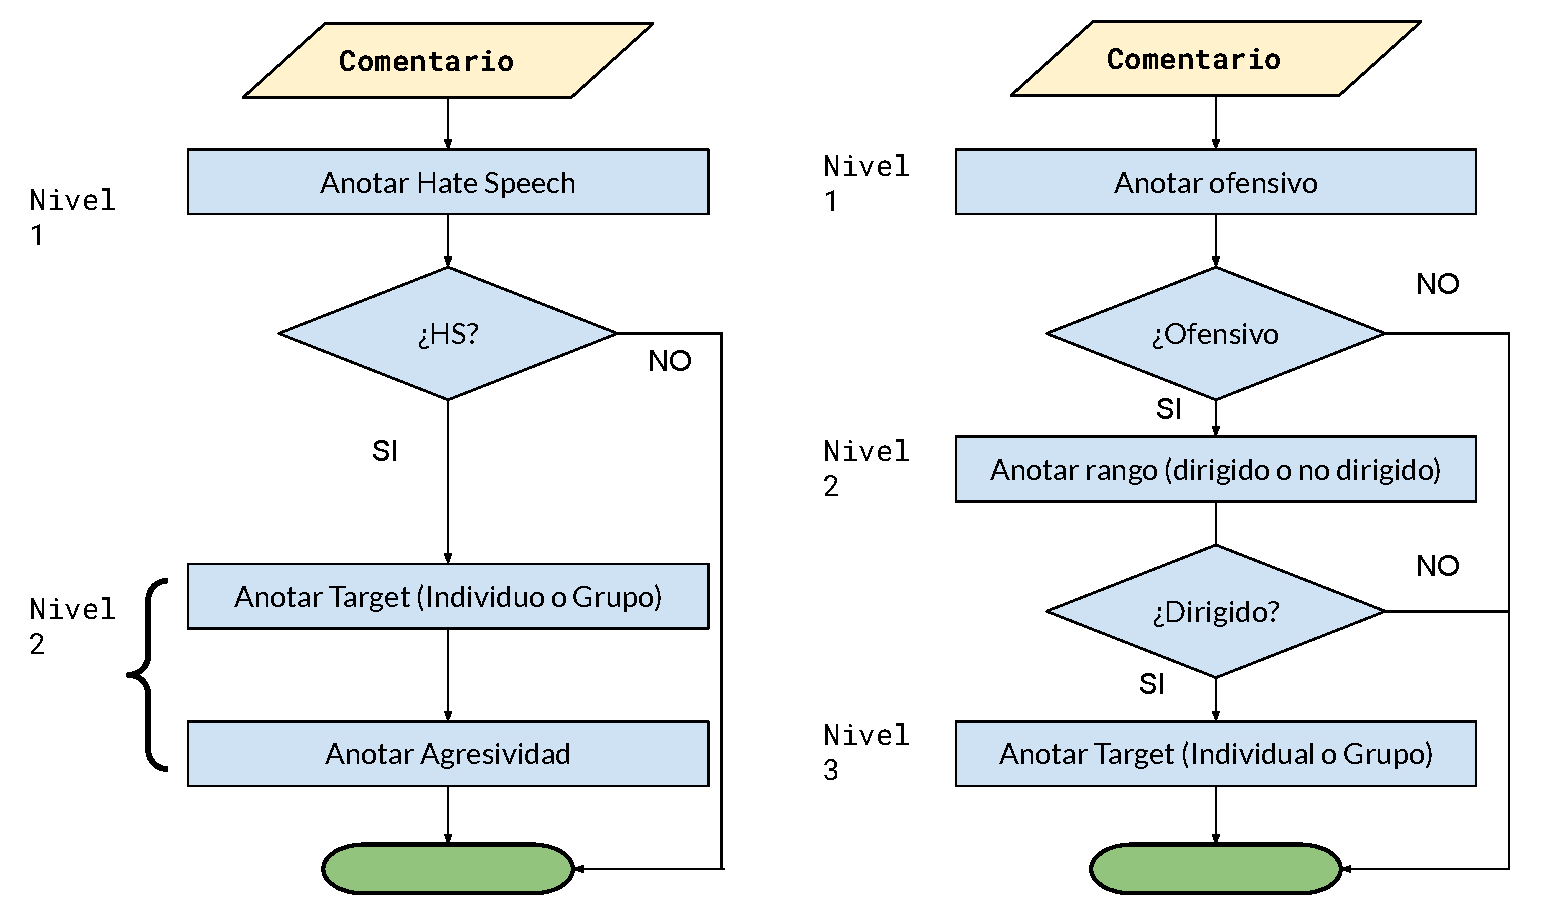
\includegraphics[width=\textwidth]{img/05/modelos_jerarquicos.pdf}
    \caption{Modelos jerárquicos de anotación. A la izquierda, tenemos el modelo jerárquico propuesto para HatEval \cite{hateval2019semeval}, a la derecha el modelo propuesto para OffensEval \cite{zampieri2019semeval2019}}
    \label{fig:modelos_offenseval_hateval}
\end{figure}


Un modelo de anotación es una representación práctica del objetivo de este proceso; es decir, del fenómeno que queremos capturar \cite{pustejovsky2012natural}. En base a la discusión del capítulo anterior, es de interés marcar comentarios discriminatorios de manera granular de modo de tener información de qué grupos y/o características se está ofendiendo. Para identificar formas más graves de discurso de odio, también es de interés identificar llamados a tomar alguna acción (violenta o no violenta) contra esa persona o grupo.

\citet{zampieri2019predicting} introdujeron un modelo jerárquico de anotación para la tarea de lenguaje ofensivo, utilizado tanto en los datasets de OffensEval \cite{zampieri2019semeval2019} y HatEval \cite{hateval2019semeval}. La idea de este modelo es realizar anotaciones en varios niveles, sólo marcando algunas variables de acuerdo a las respuestas del nivel anterior. Por ejemplo, en el caso de \hateval{}, tenemos un primer nivel que consta de marcar si un tweet contiene o no discurso de odio. Si el tweet tiene discurso de odio, entonces se anota en primer lugar si está dirigido a un individuo o a un grupo, y también si es agresivo o no. En el caso de \emph{OffensEval}, primero se anota si es ofensivo, y en caso de serlo, se marca si está dirigido a un individuo o grupo o es un insulto no dirigido. Por último, si es dirigido y ofensivo, marcamos si su objetivo es un grupo o un individuo. La Figura \ref{fig:modelos_offenseval_hateval} ilustra en modo de diagrama de flujo el modelo de anotación de ambos conjuntos de datos.


%
%
% Link: https://docs.google.com/drawings/d/14TKSC4QmZhksnlFvQcHUaZup-q3AL0Up1cNKJUr5toI/edit
%



\begin{figure}[t]
    \centering
    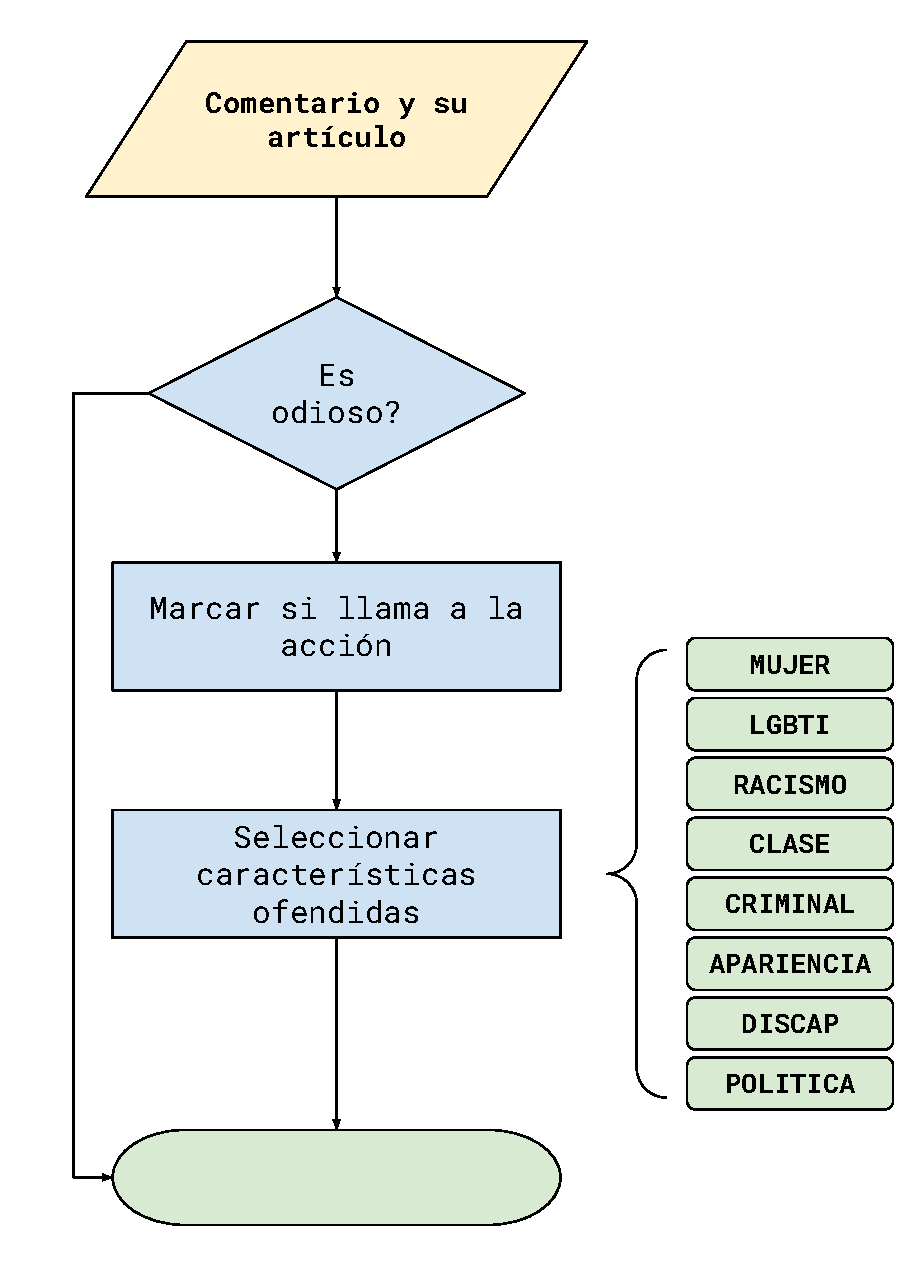
\includegraphics[width=0.5\textwidth]{img/05/annotation_model.pdf}
    \caption{Modelo de anotación para el dataset construido en este capítulo. El modelo jerárquico consta de dos niveles: el primero, donde se anota si es odioso. El segundo consta de anotar --en caso de haber sido marcado como odioso-- si contiene un llamado a la acción y a qué características ofende.}
    \label{fig:annotation_model}
\end{figure}


Basándonos en esta estructura jerárquica planteamos nuestro modelo, ilustrado en la Figura \ref{fig:annotation_model}. Para cada comentario y su respectivo contexto (el artículo), requerimos una anotación para decidir si el comentario es odioso o no. Si no es odioso, no se necesita más información. En caso de haberse marcado como odioso, el par artículo-comentario debe contener, además, una anotación por si llama o no a la acción, y al menos una categoría protegida marcada como ofendida.


\subsection{Etiquetadores}

%
% Chequear https://docs.google.com/spreadsheets/d/1PaOVw_tKVRvjZIqRl2YKnaNsvX5tHJjjY0CV9PLrc6g/edit?resourcekey#gid=366330815
%

\begin{table}[b]
    \centering
    \small
    \begin{tabularx}{\textwidth}{l l l l l l l l}
        Género& Edad  & Estudios    & Área          & Identificación    & ¿Activista?   & Experiencia\\
        \hline
        F    & 25-30  & Doctorado*  & Psicología    & Mujer             & No                   & Sí         \\
        NB   & 30-35  & Grado*      & Artes         & LGBTI             & No                   & No         \\
        F    & 30-35  & Grado*      & Antropología  & Mujer, LGBTI      & Feminista            & Sí         \\
        M    & 35-40  & Grado       & Sociología    & No                & No                   & No         \\
        F    & 35-40  & Doctorado   & Psicología    & Mujer             & No                   & No         \\
        F    & 30-35  & Grado       & Comunicación  & No                & Migrantes            & No         \\
        \hline
    \end{tabularx}
    \caption{Información sobre los anotadores. En el caso de estudios, * indica en curso. Indentificación se refiere a si se autopercibe como perteneciente de una característica protegida considerada en este trabajo. Experiencia se refiere a haber etiquetado previamente otros conjuntos de datos. }
    \label{tab:informacion_sobre_anotadores}
\end{table}

A diferencia de otros trabajos de detección de discurso de odio, decidimos garantizar que nuestros anotadores estuvieran más cerca culturalmente al problema en cuestión. El discurso de odio tiene un fuerte componente cultural, muchas veces expresado a través de jerga o expresiones dialectales muy particulares, y está relacionado con noticias muy propias de esta región. Es por esto que decidimos buscar por nuestros propios medios perfiles alineados a estos puntos y no depender de plataformas externas de crowdsourcing para esta tarea.

Reclutamos etiquetadores hablantes nativos de español rioplatense, estudiantes o graduados/as de carreras de ciencias sociales, humanidades o afines -- como ser Psicología, Sociología, Comunicación, Artes, Antropología. Para evitar sesgos en la tarea, nos interesó que no tuvieran conocimientos de inteligencia artificial o ciencia de datos. Por último, también fue de interés que sean usuarios asiduos de redes sociales para poder captar las sutilezas del lenguaje en ese medio.

El proceso de reclutamiento constó de una breve entrevista donde corroboramos que los etiquetadores fueran hablantes nativos de español rioplatense, a la vez que les describimos la tarea que debían realizar y la herramienta correspondiente de etiquetado. Luego de la entrevista, se les solicitó hacer una prueba paga que constó de leer el manual de etiquetado y anotar 10 artículos. Esto fue realizado para corroborar la calidad de los etiquetadores, aunque no rechazamos ningún postulante en este proceso. La Tabla \ref{tab:informacion_sobre_anotadores} brinda información desagregada sobre los seis etiquetadores contratados para la tarea. Los etiquetadores reclutados tienen un perfil altamente escolarizado, y dos de quienes contratamos con experiencia previa en la tarea de anotación. Un punto adicional a marcar es que dos de las etiquetadoras eran activistas --al momento de realizarse el estudio-- en organizaciones relacionadas a alguno de los grupos vulnerados que estudiamos en este trabajo.

Luego de la entrevista, se les dio una devolución de su anotación y se les reasignaron cinco de los artículos seleccionados junto a diez más (15 en total) para su anotación a modo de entrenamiento. Este fue el único conjunto de artículos que fue anotado por la totalidad de los anotadores. Al finalizar esta etapa, se les brindó una nueva devolución para ajustar el criterio de anotación, y se procedió a la etapa de anotación del dataset.

\subsection{Esquema de anotación}


%%
%%
%% Link a Google Draw:
%% https://docs.google.com/drawings/d/1esS9tAwpPVydohxd-B-xwVdAaPQRVGAo0MruBrgSKig/edit
%%
%%

\begin{figure}
    \centering
    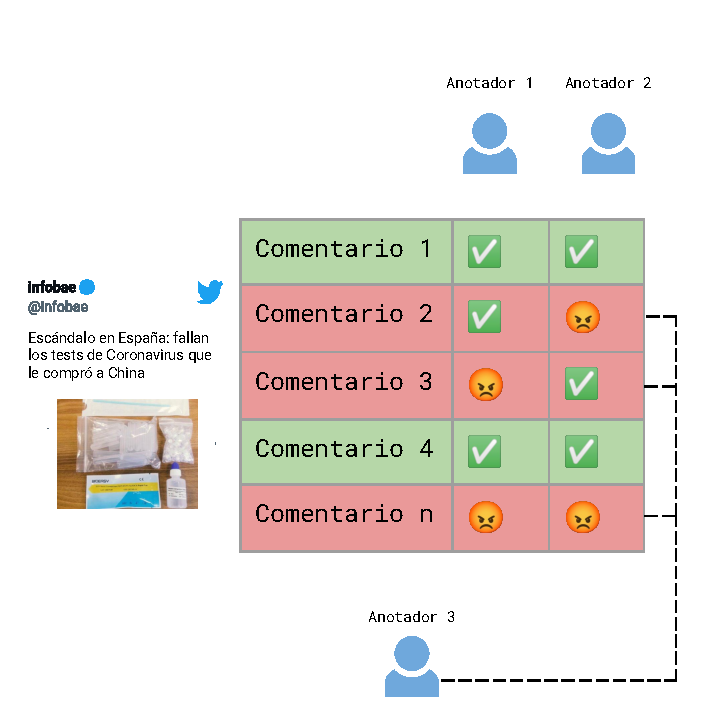
\includegraphics[width=\textwidth]{img/05/esquema_anotacion.pdf}
    \caption{Esquema de anotación. Caso en que ambos anotadores etiqueten los comentarios del artículo}
    \label{fig:annotation_schema}
\end{figure}

Pasamos ahora a describir la mecánica del proceso de anotación. Para lo que respecta a este trabajo, tomamos como la unidad de anotación al artículo. Cada etiquetador, al serle presentado un artículo, tuvo dos opciones: etiquetarlo o saltearlo. En caso de decidir etiquetarlo, tuvo que marcar las etiquetas correspondientes a cada uno de los comentarios del artículo de acuerdo al modelo descripto. La idea de permitir el salteado fue doble: evitar contenido poco interesante en términos de comentarios discriminatorios, y también dar la posibilidad al trabajador de evitar contenido sensible o perturbador para su persona.

Considerando la dificultad de la tarea y los límites borrosos del discurso de odio, decidimos seguir un esquema de etiquetado similar al de trabajos previos donde múltiples personas anotan una misma instancia. Una posibilidad considerada en un principio fue asignar el artículo completo a tres anotadores; sin embargo, esta modalidad sería ineficiente dada la baja cantidad de contenido discriminatorio observada preliminarmente entre los comentarios seleccionados. Decidimos entonces ir por un esquema de desempate similar al de \citet{hateval2019semeval}: dos personas anotan un artículo, y luego un tercero anota sólo aquellos comentarios donde al menos uno marcó que existe contenido odioso. Esta modalidad permite que haya una tercera anotación incluso cuando las dos previas marcaron contenido odioso, siendo esto realizado para recolectar más información sobre los comentarios. Dada la incidencia de comentarios odiosos (que veremos luego en los resultados) la adición de esta tercera etiqueta en estos casos técnicamente innecesarios tuvo un bajo costo.



%%
%%
%% Link a Google Draw
%% https://docs.google.com/drawings/d/1TOlCgZggCmYHgZWV7ZrIIlXuhcFUMeYw4PcFM7XdY2k/edit
%%
%%

\begin{figure}
    \centering
    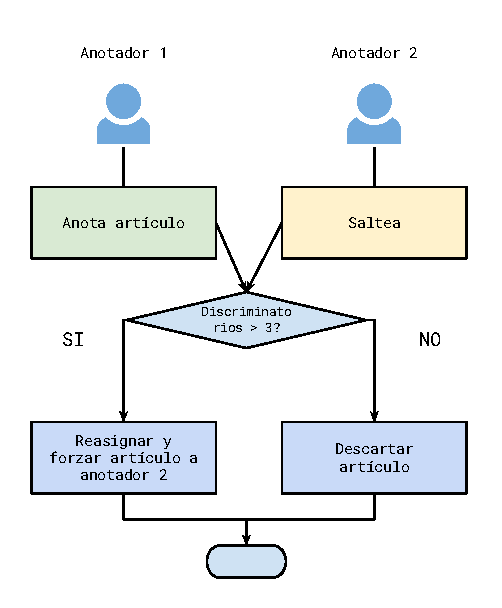
\includegraphics[width=0.5\textwidth]{img/esquema_anotacion_caso_2.pdf}
    \caption{Esquema de anotación. Caso en que un anotador decida saltear}
    \label{fig:annotation_schema_case_two}
\end{figure}


La Figura \ref{fig:annotation_schema} ilustra el flujo en el caso de que ninguno de los anotadores asignados decida saltear el artículo. Ahora ¿qué pasa si alguno de los dos anotadores decide saltear el artículo?

\begin{enumerate}
    \item Si los dos etiquetadores asignados deciden pasar por alto el artículo asignado, entonces lo descartamos del conjunto de datos
    \item En el caso de que uno lo saltee y el otro lo anote y encuentre menos de 4 comentarios odiosos, entonces también descartamos el artículo
    \item En el caso de que uno lo saltee y el otro lo anote encontrando cuatro o más comentarios odiosos, entonces reasignamos el artículo al etiquetador que salteó, sin darle esta vez posibilidad a que no lo anote
\end{enumerate}

Tomamos la decisión de descartar los artículos en los dos primeros casos intentando maximizar la tasa de comentarios discriminatorios encontrados. En caso de reasignar el artículo, revocamos la posibilidad de saltearlo \footnote{Teniendo en cuenta la posibilidad de que hayan salteado por contenido perturbador para el anotador, dimos la posibilidad de que nos avisen que no querían trabajar en ese artículo. No hubo problemas al respecto de todas formas}. La Figura \ref{fig:annotation_schema_case_two} ilustra el esquema de anotación de artículos recién descripto, que se complementa con el de la Figura \ref{fig:annotation_schema}.



%Con este esquema, y teniendo en cuenta los números finales obtenidos del dataset, dedicamos 2.16 etiquetados por comentarios versus 3 etiquetados por comentario de anotar tres veces todo.


Como resultado de este esquema, cada comentario de nuestro dataset puede tener dos o tres anotaciones, siendo los casos posibles los siguientes:

\begin{enumerate}
    \item Dos anotaciones negativas: es decir, que no encuentran discurso de odio en el comentario
    \item Tres anotaciones, con al menos una que marque el comentario como odioso
\end{enumerate}


%
% Esto quizás va después
%
\subsection{Herramienta de etiquetado}

%%
%% Link a Google Draw: https://docs.google.com/drawings/d/1E24-2l6hsNj2JSKBZOD8QvZCJR6rrGjz-cWwt8XuPRg/edit
%%

\begin{figure}
    \centering
    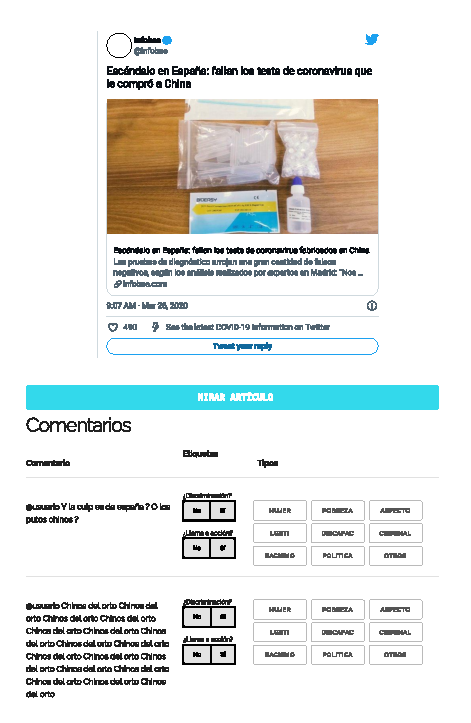
\includegraphics[width=\textwidth]{img/labeler.pdf}
    \caption{Pantalla del etiquetador}
    \label{fig:labeler_example}
\end{figure}

Al no optar por utilizar servicios de etiquetado tercerizado, desarrollamos nuestra propia aplicación para esta tarea. Cada etiquetador tuvo acceso a un sitio web donde se le mostraron uno a uno los artículos asignados, de acuerdo al orden establecido por los administradores de la aplicación. La Figura \ref{fig:labeler_example} ilustra la interfaz de anotación presentada a los usuarios del sistema. Cada artículo es presentado junto a su tweet correspondiente, al texto replegado de la noticia --en caso de que un usuario requiera su lectura-- y a los comentarios.

Ante esto, el etiquetador puede elegir saltear el artículo o etiquetarlo. Si decide etiquetarlo, debe para cada comentario marcar usando un control de tipo interruptor:

\begin{enumerate}
    \item Si el comentario contiene discurso discriminatorio.
    \item En caso de ser discriminatorio, marcar si llama a la acción.
    \item En caso de ser discriminatorio, marcar al menos una característica ofendida.
\end{enumerate}

Para el desarrollo de la aplicación usamos \emph{Django} \footnote{\url{https://www.djangoproject.com/}}, un framework de Python para desarrollo web, y Javascript plano. Como base de datos utilizamos \emph{SQLite}, ya que el sistema no tuvo grandes requerimientos de concurrencia (sólo seis o siete usuarios simultáneos).


Cada tweet fue presentado con un preprocesado básico que consistió en reemplazar handles de usuarios por un token especial \verb|@usuario| para evitar cualquier sesgo. Por ejemplo, si un usuario A conocido como difusor de discurso discriminatorio retwittea la noticia y otro responde a ese retweet, en el tweet aparece el nombre de A, lo cual podría condicionar a quien tenga que evaluar ese comentario.


\subsection{Asignación}

Llamamos \tbf{asignación} al procedimiento de colocar \tbf{etiquetas} (también llamadas \emph{gold labels}) a las instancias de nuestro conjunto de datos \cite{pustejovsky2012natural}. El modelo descripto en la Sección \ref{sec:modelo_etiquetado} consta de una etiqueta binaria que marca si el contenido es discriminatorio o no (notamos HS) en el primer nivel, y luego 9 etiquetas binarias para el segundo: una para las llamadas a la acción (notamos CALLS) y otras ocho para las características ofendidas listadas en la Tabla \ref{tab:caracteristicas_protegidas}. Recordemos que una anotación negativa sólo consta de HS negativo, mientras que una positiva consta de un HS positivo, una etiqueta para CALLS y al menos una etiqueta positiva de las características ofendidas.

Pensamos el proceso de asignación de etiquetas como una votación, donde cada anotador da un voto para cada variable a asignar. Detallamos a continuación cómo fueron asignadas las etiquetas del conjunto de datos:

\begin{enumerate}
    \item Para la etiqueta de HS, asignamos mediante votación mayoritaria: 2 o más votos para HS positivo, caso contrario HS negativo.
    \item En caso de haber marcado que hay HS: marcamos CALLS es positivo por votación mayoritaria.
    \item En caso de haber marcado que hay HS: marcamos como positivas todas aquellas características marcadas por los anotadores.
\end{enumerate}

La primer decisión es la más obvia y razonable: para que un comentario sea considerado como odioso (HS positivo) tiene que ocurrir que al menos dos etiquetadores lo marquen como tal. Si se anota HS positivo, para que CALLS sea positivo tiene que haber al menos dos votos en tal sentido. Si un anotador marcó que hay llamado a la acción y otro que no, asignamos CALLS negativo. \todo{Acá Agus pregunta por qué no asignamos CALLS si al menos uno marca. Me parece que no es la idea: corresponde que haya cierto consenso sobre que está dado este fenómeno. Con el mismo criterio, deberíamos marcar así HS}

En el caso de las características no realizamos votación mayoritaria, sino que la anotamos si al menos un etiquetador lo hizo. Esta decisión podría haberse tomado de otra manera; por ejemplo, sólo tomando aquellos casos donde haya cierto grado de coincidencia entre los comentarios. Sin embargo, al considerar que los límites entre las características son difusos (por ejemplo, APARIENCIA y MUJER tienen una intersección no nula y a veces CLASE y RACISMO también) preferimos anotarlas de esta manera.


\section{Resultados}

\begin{table}
    \centering
    % \begin{tabular}{lrr}
    %     \toprule
    %     Total articles & 1238    \\
    %     Total comments &  56869  \\
    %     Hateful Tweets &   8715  \\
    %     Ratio          &   0.153 \\
    % \end{tabular}
    \begin{tabular}{lrr}
        \toprule
        Característica &  Número &  Llamadas a acción \\
        \midrule
        RACISMO        &   \num{2469} & \num{ 674} \\
        APARIENCIA     &   \num{1803} & \num{  34} \\
        CRIMINAL       &   \num{1642} & \num{ 722} \\
        POLITICA       &   \num{1428} & \num{ 136} \\
        MUJER          &   \num{1332} & \num{  18} \\
        CLASE          &   \num{ 823} & \num{ 135} \\
        LGBTI          &   \num{ 818} & \num{  11} \\
        DISCAPACIDAD   &   \num{ 580} & \num{   4} \\
        TOTAL          &   \num{8715} & \num{1451} \\
        \bottomrule
    \end{tabular}
    \caption{Datos desagregados por característica de los comentarios discriminatorios del conjunto de datos resultante. Se listan además la cantidad de llamados a la acción dentro de cada una. Notar que el total no corresponde con la suma de las columnas ya que un mismo comentario puede estar asignado a más de una característica.}
    \label{tab:dataset_figures}

\end{table}

El conjunto resultante consta de \num{1238} artículos etiquetados, y \num{56869} comentarios respectivamente, de los cuales \num{8715} contienen contenido discriminatorio según los criterios de asignación antes referidos. Aproximadamente 1 de cada 6 comentarios es discriminatorio, aunque vale aclarar que esto no es representativo del universo de notas periodísticas ya que la selección de los datos no fue aleatoria.

\todo{cambiar todos los números al comando num}

La Tabla \ref{tab:dataset_figures} contiene los números de los comentarios anotados y desagregados por las distintas características consideradas y los llamados a la acción. La categoría con más comentarios es RACISMO, seguido por APARIENCIA y CRIMINAL. Dentro de los tweets que llaman a algún tipo de acción, se coloca en primer lugar los dirigidos hacia la categoría CRIMINAL, muchos en la forma de llamados a matar a criminales y delincuentes. La categoría RACISMO acapara también muchos llamados a la acción, mayormente contra población china a la que se culpa de la pandemia del COVID-19 y conteniendo llamados a tomar distintas sanciones contra sus integrantes.


\begin{table}
    \centering
    \begin{tabular}{lc}
        \toprule
        Categoría   & $\alpha$  \\
        \midrule
        Discurso de odio     &  \num{0.58} \\
        Llamados a la acción &  \num{0.64} \\
        \hline
        MUJER                &  \num{0.78} \\
        LGBTI                &  \num{0.92} \\
        RACISMO              &  \num{0.93} \\
        CLASE                &  \num{0.71} \\
        POLITICA             &  \num{0.81} \\
        DISCAPACIDAD         &  \num{0.85} \\
        APARIENCIA           &  \num{0.87} \\
        CRIMINAL             &  \num{0.93} \\
        \bottomrule
    \end{tabular}
    \caption{Tabla de acuerdo para la etiqueta de discurso de odio y diferentes características medido por $\alpha$ de Krippendorff. El acuerdo sobre \emph{discurso de odio} es reportado sobre todos los etiquetadores que hayan analizado cada comentario. Para el resto de las características, el acuerdo es calculado sólo sobre aquellas anotaciones que marcaron discurso de odio.}
    \label{tab:annotation_agreement}
\end{table}

La Tabla \ref{tab:annotation_agreement} reporta el acuerdo entre anotadores usando la métrica \emph{alfa de Krippendorff} \cite{krippendorff2018content}. Esta métrica mide el acuerdo entre diversos anotadores, donde $1$ es acuerdo total, y 0 o valores negativos indican ningún tipo de acuerdo. Puede entenderse como una generalización de la métrica \emph{kappa de Fleiss} para el caso en que los anotadores no etiqueten todas las instancias. Utilizamos para su cálculo la implementación en Python de la librería \emph{krippendorff} \footnote{\url{https://github.com/pln-fing-udelar/fast-krippendorff}}.

Reportamos en primer lugar el acuerdo para HS sobre todas las etiquetas. En el caso de las etiquetas del segundo nivel del modelo jerárquico (características y llamado a la acción) calculamos el acuerdo sólo sobre aquellas que hayan marcado que el comentario contiene discurso de odio. Esto es equivalente en términos del cálculo propuesto en \citet{krippendorff2018content} a calcular el acuerdo con una etiqueta faltante en el segundo nivel para aquellos anotadores que hayan marcado que no hay HS.

Si bien el acuerdo sobre cada característica tiende a ser alto, debe leerse como el acuerdo sobre la razón detrás del discurso de odio. La mayor penalización queda reservada a la etiqueta de discurso de odio que tiene $\alpha = 0.58$, algo que podría marcarse como un acuerdo razonable teniendo en cuenta valores observados en la literatura \cite{poletto2021resources}.



\subsection{Co-ocurrencia de características ofendidas}
%%
%%
%% Generar con
%% https://docs.google.com/drawings/d/1IcBITgNJN-tehmvnZqcSF9cUuWIpNKJg6yHI5yjNF9c/edit
%%
%%

\begin{figure}[t]
    \centering
    \begin{subfigure}[]{0.49\textwidth}
        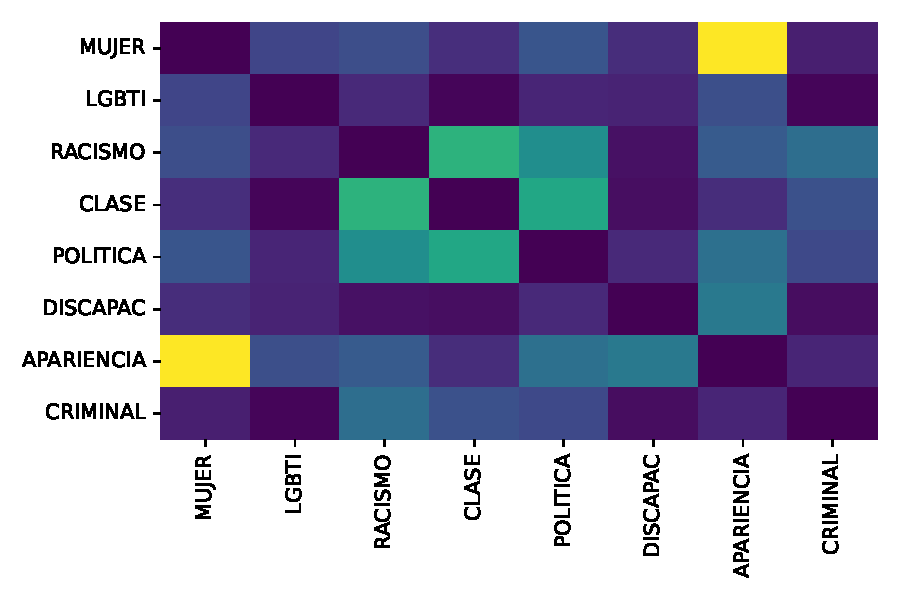
\includegraphics[width=\textwidth]{img/05/heatmap_characteristics.pdf}
        \caption{Co-ocurrencia de las características ofendidas en un comentario}
        \label{subfig:heatmap_characteristics_comment}
    \end{subfigure}
    \begin{subfigure}[]{0.49\textwidth}
        \centering
        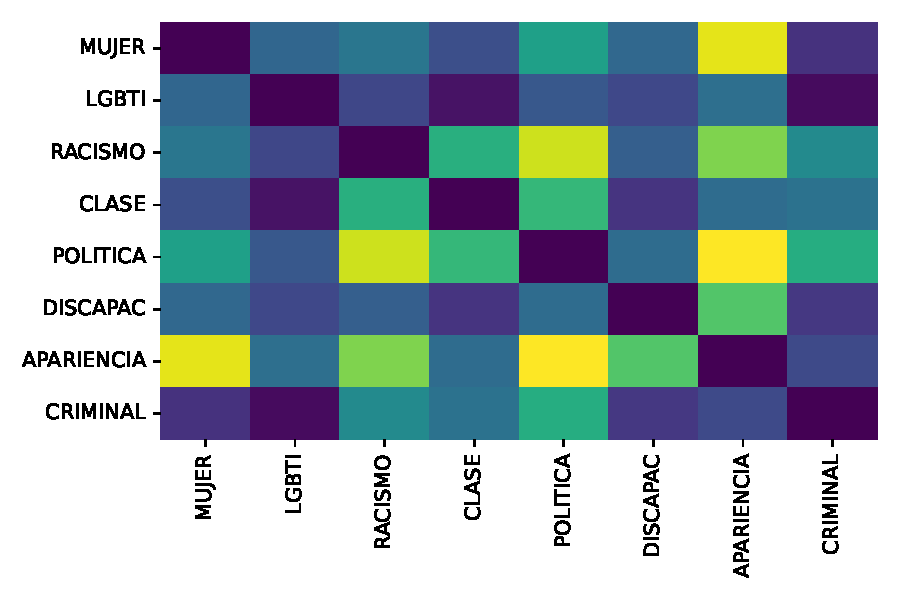
\includegraphics[width=\textwidth]{img/05/heatmap_characteristics_article.pdf}
        \caption{Co-ocurrencia de las características ofendidas en un artículo}
        \label{subfig:heatmap_characteristics_article}
    \end{subfigure}

    \caption{Matrices de co-ocurrencias de características ofendidas. La figura \ref{subfig:heatmap_characteristics_comment} muestra la co-ocurrencia dentro de un mismo comentario, y la figura \ref{subfig:heatmap_characteristics_article} muestra la co-ocurrencia dentro de los comentarios de un mismo artículo. Más luminoso indica más co-ocurrencia}
    \label{fig:heatmap_characteristics}
\end{figure}


De los \num{8715} comentarios odiosos, el 77\% de ellos (\num{6777}) contiene una sola característica ofendida de acuerdo al proceso de asignación realizado. Cerca del 20\% tienen dos características ofendidas, y 220 comentarios tienen tres o más. La Figura \ref{fig:heatmap_characteristics} ilustra la matriz de co-ocurrencia entre las distintas características para aquellos comentarios que tengan más de una característica ofendida. En ella podemos ver que la máxima co-ocurrencia se da entre las características MUJER y APARIENCIA, seguidos por RACISMO y CLASE, POLITICA y CLASE, y RACISMO y POLITICA.



Otra forma de analizar la co-ocurrencia es agrupando por artículos las distintas características de sus comentarios, para así observar como un mismo contexto puede suscitar distintos tipos discriminación. La Figura \ref{subfig:heatmap_characteristics_article} ilustra las interacciones entre las distintas características por artículo. Puede observarse en esta figura mayor dispersión en las co-ocurrencias que en la Figura \ref{subfig:heatmap_characteristics_comment}, apreciándose algunas interacciones adicionales como por ejemplo entre RACISMO y POLITICA y --quizás inesperadamente-- entre APARIENCIA y POLITICA. La característica que parece tener menos interacción con las demás es LGBTI, indicando que está bien delimitada de las demás posibles causas de discurso discriminatorio.

\begin{table}[t]
    \small
    \begin{tabular}{l p{0.3\textwidth} p{0.5\textwidth}}
        \toprule
        Índice & Contexto        & Comentario \\
        \midrule
        \rule{0pt}{3ex}1 & Ofelia Fernández apoyó al Gobierno en la polémica por los presos y apuntó a la Justicia que ``odia a las mujeres''  & Hijadept,, ojala pronto recibas la visita de alguno de esos gusanos. Te van a quedar. Ganas de apoyar al. Gobierno? Larva rastrera gorda. Decerebrada\\%& MUJER, POLITICA, APARIENCIA, DISCAPACIDAD \\
        \rule{0pt}{3ex}2 & ``Es hora de ponerle límites al odio'' | Por Victoria Donda &  Justo ésta zurda mugrienta, ignorante y altanera... \\% & MUJER, POLITICA, APARIENCIA\\
        \rule{0pt}{3ex}3 &Coronavirus en la Argentina: un video pone en evidencia la violación de la cuarentena en la Villa 1-11-14 & Cierren esa nido de negros y napalm. Hasta reducís el crimen y el gasto público.\\%& CLASE, RACISMO\\
        \rule{0pt}{3ex}4 & Fabiola Yáñez denunció a un periodista por publicaciones agraviantes & Claro si ofendel a la que se cuelga en el caño xq ahora cree ser primera dama?😂 hay que ser peruka para dar asco y ser basuras bigote enseguida ordena como se metió en Facebook y en todo que culpa te.emos que saque la mujer del cabarute? \\ % RACISMO, MUJER
        \rule{0pt}{3ex}5 & Los infectados en villas porteñas crecieron un 80\% en cuatro días & Ojalá que el virus penetre más en las villas y maten a todos esos delincuentes que viven ahi, hay paraguayos narcos, bolivianos que traen la droga de bolivia, y gente de mala vida. También hay travas que van a trabajar de noche a palermo.\\%& RACISMO, CLASE, LGBTI  \\
        \rule{0pt}{3ex}6 & El enojo de Moria Casán contra Rocío Oliva: ``Mucha agua oxigenada, le quedó media neurona para jugar a la pelota'' & Y la vieja Moria, mucha cirugía y estiramiento. de cara que parece un travesti \\
        \rule{0pt}{3ex}7 & Ricky Martin: ``Soy un hombre latino y homosexual viviendo en los Estados Unidos, soy una amenaza'' & Ridículo perdiste tú rumbo das náuseas 🤮 famosos eternos (víctimas) 🙄🤦‍♀️ ándate a Puerto Rico entonces ahí no serás una amenaza\\ %& LGBTI, RACISMO
        \hline
    \end{tabular}
    \caption{Ejemplos con más de una característica ofendida marcada}
    \label{tab:multi_char_examples}
\end{table}




La Tabla \ref{tab:multi_char_examples} muestra algunos ejemplos con más de una característica ofendida. Algunos de los comentarios se encuentran en la frontera de las características, como por ejemplo, APARIENCIA y MUJER en los ejemplos 1 y 2, o CLASE y RACISMO en el ejemplo 3. Otras instancias son conjunciones de expresiones discriminatorias, como en el caso del número 5, donde tenemos una conjunción de RACISMO, CLASE, y LGBTI; o bien en el comentario 6, de APARIENCIA y LGBTI.



\subsection{Análisis por característica}
\label{sec:analisis_dataset_por_caracteristica}
\todo{highlight a la tabla y sus palabras ofensivas}
\begin{table}
    \scriptsize
    \centering
    \begin{tabular}{p{0.1\textwidth} p{0.45\textwidth} p{0.40\textwidth}}
        \hline
        Tipo & Contexto & Texto \\
        \hline
        %WOMEN & Nicole Neumann apuntó contra los consumidores de carne: “Sigan comiendo asadito” & @usuario Debieras comerte uno así te sacas esa cara agria que tenes🤣🤣👎 \\
        \mr{12}{MUJER} & Por el mundo: Florencia Peña mostró su lujosa nueva casa con bar, muelle y pileta & @usuario Cuando succionas las correctas \\
         & El exabrupto de Rodolfo Barili con una modelo que se metió en el baúl de un auto para violar la cuarentena & @usuario Barili, ojo es mujer, en cualquier momento te caen las hordas de feminazis, pero estoy al 100\% CON VOS!! \\
         & Video: tres mujeres forzaron la puerta de un edificio en Palermo y desvalijaron dos departamentos & @usuario 3 feministas , claramente es el perfil de las feministas \\
         & Británica llegó a Perú por 10 días y se quedó por amor: vive sin agua potable y entre insectos & @usuario Pero empomada todo el día... \\
         & “Me esterilicé, pero no odio a los niños”: mi vida dentro del movimiento “libre de hijos” & @usuario Es que sos incogible..quien te va a hacer un hijo.....algun ciegoooo \\
         & Mia Khalifa: actuó en videos porno durante pocos meses, cobró fama mundial y ahora lucha por borrar su pasado & @usuario JAJAJAJAAJAJAAJA SEGUILA CHUPANDO.... \\
         & ¿Se puede ser feminista y llorar a Diego Maradona? & @usuario Para las feminazis toda ilógica es correcta \\
         & Claribel Medina, indignada con un grupo de personas reunidas en un bar: “La gente está sin barbijo mientras los actores no podemos trabajar” & @usuario La menopausia nos pone locas 🤦🏽‍♀️🤣 \\
         & Narda Lepes: “Mil veces me tocaron el culo en las cocinas de los restaurantes” & @usuario Tenes lindo culo? \\
         & Un policía se defendió de un robo en Pompeya, mató a un ladrón y estuvo dos días preso & @usuario Que jueza hija de mil puta ojalá t afanen a vos y t maten un ser querido a ver qué haces LLEGUA de mierda puta \\
         & “Cristian, mirá lo que hago por vos”: quién es la modelo que se metió en el baúl de un auto para violar la cuarentena & @usuario Jajaja modelo Hot jaja Telosu!! Mami diría la Moria !! Jaja ridícula tafaldegaver \\
         & La aberrante arenga machista que dio el preparador físico de Güemes de Santiago del Estero & @usuario Que aliade te volviste Clarín, vos te culeas la que tiene olor a pingo (feminazi) \\
        \hline
        \hline
        \mr{8}{LGBTI} & Por qué Flor de la V no continuó en Mujeres de eltrece, tras la salida de Claudia Fontán & @usuario y..porque no es mujer, más claro echale agua \\
         & Histórico: Mara Gómez fue habilitada y será la primera jugadora trans en el fútbol argentino & @usuario Unos huevos bárbaros tiene esta mina!!!!! \\
         & La historia de la modelo colombiana trans que besa la panza de su esposo embarazado de ocho meses & @usuario Un macho besando a otro macho \\
         & Luis Novaresio le dedicó un romántico mensaje a Braulio Bauab por su cumpleaños & @usuario Guacale \\
         & Eugenio Zaffaroni le contestó a Sergio Berni tras la polémica por las domiciliarias: “Es el populacherismo vindicativo que llenó las cárceles” & @usuario cuando se muere este viejo trolo enfermo \\
         & La impactante historia de la tenista trans que hoy es la N° 3 de Argentina en la categoría senior femenino & @usuario Vergonzoso que  las mujeres toleren esto.\textbackslash nEse tenista debería jugar con hombres o a lo sumo, en un torneo de sujetos como él. \\
         & Joe Biden nominó a Rachel Levine, una mujer transgénero, para que sea su subsecretaria de Salud & @usuario Este presidente es la dejeneracion total del mundo \\
         & Así luce el actor Elliot Page tras declararse trans & @usuario Tiene Bija? No. Tiene Concha? Si. Es mujer entonces \\
         & El abuelo que a los 90 años confesó: “Soy gay, soy libre y estoy afuera” & @usuario Como no te agarra el Coronavirus.   🤮🤮 \\
        \hline
    \end{tabular}

    \caption{Ejemplos discriminatorios del dataset contra mujeres y la comunidad LGBTI.}
    \label{tab:women_and_lgbti_examples}
\end{table}


\begin{table}
    \scriptsize
    \centering
    \begin{tabular}{p{0.1\textwidth} p{0.45\textwidth} p{0.40\textwidth}}
        \hline
        Tipo & Contexto & Texto \\
        \hline
        \mr{9}{RACISMO} & Coronavirus: las terribles imágenes del mercado donde se originó la pandemia & @usuario Hay que matarlos hijos de puta 😑 \\
         & Malestar en Washington con el Gobierno argentino porque no dejó atracar al buque más moderno de la guardia costera de Estados Unidos & @usuario Amo ver los sudacas que se creen yankis enojados por esto. \\
         & Milagro Sala: “Seguimos presos, los que nos gobiernan tienen que cambiar las cabezas” & @usuario Negra, seguis presa por chorra. \\
         & Al menos 7 muertos en China a causa de un virus transmitido por garrapatas & @usuario Que no venga ningún chino más a la Argentina! Por favor! Ya Basta! \\
         & En China comenzó el tradicional Festival de Carne de Perro a pesar de la pandemia de coronavirus y una ONG intenta salvarlos & @usuario No soy racista, pero hay que matar a todos los chinos \\
         & Científicos identificaron en China otro virus respiratorio “con potencial para convertirse en pandemia” & @usuario Nos infectan a Todos!!! \\
         & Coronavirus. Yanzhong Huang: "Es bastante probable que ya se esté gestando un Covid-21" & @usuario Bombas urgente a esta maldita raza \\
         & Denunciaron la nueva maniobra de China para ocultar las verdaderas cifras del coronavirus & @usuario Mundialmente mantenemos china xq todo viene de ahí y hoy estamos fundidos y en emergencia... \#ChinaVirus no quiero ver un \#chino x mucho tiempo! \\
         & Villa Mascardi: impresionante operativo con tanquetas blindadas para que una fiscal ingresara a una zona controlada por mapuches & @usuario Basta!!! No son mapuches son delincuentes !!! A ver si alguien pone las pelotas donde hay que ponerlas y los cagan a tiros de una vez !!! \\
        \hline
        \hline
        %\rotatebox[origin=c]{90}{rota}
        \mr{5}{CRIMINAL} & Aberrante: un político de Misiones admitió haber esclavizado y violado a sus tres hijastras & @usuario Solo se requiere una bala. \\
         & Rosario: un grupo de vecinos linchó y mató a golpes a un joven acusado de robar autos & @usuario esta perfecto, ejemplo a los demás \\
         & El panadero que mató a un ladrón en La Matanza: "No soy un asesino, estoy arrepentido" & @usuario Que dice señor ! No sé arrepienta, que hizo una obra de bien.Era su vida o la del delincuente. \\
         & Video: salió de la cárcel por el coronavirus y murió de un tiro el mismo día al festejar su libertad & @usuario Justicia divina!! \\
         & Le sacó el arma al ladrón que lo asaltó, lo corrió y lo mató de un disparo: quedó detenido & @usuario Buenísimo vamos por el exterminio total de estos primates. \\
        \hline
        \hline
        \mr{8}{CLASE} & La Justicia ordenó el desalojo de la masiva toma de terrenos en Guernica & @usuario Lanzallamas y a otra cosa \\
         & Hubo tensión en la Quinta de Olivos entre un grupo que apoyaba a Alberto Fernández y manifestantes del banderazo contra el Gobierno & @usuario PLANEROS Y BARRABRAVAS \\
         & Organizaciones sociales cortaron la avenida 9 de Julio: reclamaron un salario mínimo de \$ 45.000 & @usuario Vayan a lo laburar hdp. \\
         & La historia de una familia de cartoneros en la toma de Guernica: “Por primera vez sentimos que tenemos un hogar” & @usuario Bala. \\
         & El Gobierno autorizó la apertura de las escuelas porteñas para las elecciones de Bolivia & @usuario No sería mejor deportar a los bolivianos indocumentados?.además nos suman pobreza e indigencia \\
         & Coronavirus en Argentina: un dirigente radical deseó que la pandemia “haga una limpieza étnica” con “negros de La Matanza” & @usuario Es el deseo de todo argentino de bien \\
         & El Polo Obrero realiza un corte en la Panamericana en contra de la flexibilización de la cuarentena y en reclamo de aumentos a los planes sociales & @usuario Clarísimo que no quieren laburar y quieren vivir de nosotros! \\
         & Coronavirus en la Argentina: movimientos sociales reclaman asistencia alimentaria en el Obelisco & @usuario Anda a laburar lpqtp \\
        \hline
    \end{tabular}

    \caption{Ejemplos discriminatorios del dataset por motivos de clase, racismo, o contra criminales.}
    \label{tab:class_racism_examples}
\end{table}


\begin{table}
    \scriptsize
    \centering
    \begin{tabular}{p{0.1\textwidth} p{0.45\textwidth} p{0.40\textwidth}}
        \hline
        Tipo & Contexto & Texto \\
        \hline

     \mr{5}{POLITICA} & Confirman una mutación en el coronavirus que puede hacerlo 10 veces más contagioso que la cepa original de Wuhan & @usuario ME ALEGRO MUCHÍSIMO.\textbackslash nOJALÁ LLEGUE PRONTO A ARGENTINA Y ARRASE CON TODO.\textbackslash nPODRÍAMOS VER AL FIN ALGO MÁS DAÑINO QUE EL CÁNCER PERONISTA Y SU METÁSTASIS KIRCHNERISTA. \\
      & Murió un nieto recuperado por Abuelas de Plaza de Mayo: los mensajes de Alberto Fernández y Cristina Kirchner & @usuario Un planero menos. \\
      & Última encuesta: ¿Qué mujer superó a Alberto Fernández en imagen positiva? & @usuario Les ahorro el clickbait. Es Vidal, igual perdió por 20 puntos. Gorila LTA. \\
      & Cómo es la cerveza “peronista” que el Chacho Coudet le regaló a Alberto Fernández & @usuario Debe ser meo de gato. berreta como todo lo peroncho \\
      & El descargo de Nicolás Wiñazki después de que Vero Lozano se burlara de él: “Quizás le afecta la cuarentena” & @usuario Yo creo que al revés, patético operador. Solo los gorilas pueden bancarte croto \\
      \hline
      \hline
    \mr{5}{APARIENC.} & Axel Kicillof recomendó una “cuarentena previa” de 14 días para “llegar sanos a Navidad y Año Nuevo” & @usuario Chuoame la verga enano moishe \\
     & Video indignante: piba violó la cuarentena y viajó en el baúl de un taxi para ver a un chico & @usuario Habría qur buscar también y meter en cana al cirujano que le hizo la nariz!! Parece Michael Jackson la loca!!! \\
     & El senador José Mayans defendió a Gildo Insfrán: “En pandemia no hay derechos” & @usuario Volve al gancho , docer \\
     & El video sexy de More Rial en corpiño & @usuario Asco \\
     & El sensual paseo en moto de Florencia Peña: "Próxima parada: tu casa" & @usuario Que tiene de sensual, ésta vieja cascoteada?prostituta de cuarta,kukaracha inmunda! \\

    \hline
    \hline
    \mr{4}{DISCAPAC.}& Patricia Bullrich pidió ser drásticos con los docentes: “El que no va, tendrá que ser reemplazado” & @usuario Estragos del tinto \\
      & El abuelo que a los 90 años confesó: “Soy gay, soy libre y estoy afuera” & @usuario Alhzeimer o demencia senil!!!!! \\
      & Elisa Carrió dijo que “ninguna pandemia es excusa para suspender la República” y advirtió que “vienen por los campos” & @usuario Si sacan a la paciente psquiatrica es porque están hasta las manos.\textbackslash n\#CarcelACambiemos \\
      & Florencia Kirchner y su posteo a favor de la amistad: "Nunca entendí la desesperación por la pareja" & @usuario La enfermita está mejor que yo,y no se calienta por la hija \\
    \hline
    \mr{6}{INCITACIÓN} & Harán un listado de los presos en situación de riesgo por el coronavirus para evaluar si deben salir de prisión & @usuario @usuario Todo al reves! Si hay alguno con coronavirus PONGANLO EN EL MEDIO! \\
         & La advertencia de Juan Grabois: “Van a haber 1, 5, 20 Guernicas” & @usuario @usuario Habra 100 paredones \\
         & Otro caso de peste bubónica enciende las alarmas en China & @usuario Una atómica a China... \\
         & Coronavirus: afirman que volvió la venta de carne de murciélagos en China & @usuario Boicot a todo producto chino!!! \\
         & Villa Mascardi: impresionante operativo con tanquetas blindadas para que una fiscal ingresara a una zona controlada por mapuches & @usuario El Diálogo se Inicia con BALAS y Finaliza con La Última \\
         & Coronavirus en China: la ciudad de Shenzhen prohíbe comer perros y gatos & @usuario habrá alguna manera de erradicar a estos tipos del mundo ? \\
    \hline
    \hline
    \end{tabular}
    \caption{Ejemplos discriminatorios del dataset. INCITACIÓN refiere a los llamados a realizar algún tipo de medida contra el grupo o la persona atacada. }
    \label{tab:politics_and_calls_examples}
\end{table}


Las tablas \ref{tab:women_and_lgbti_examples}, \ref{tab:class_racism_examples} y \ref{tab:politics_and_calls_examples} ilustran ejemplos seleccionados de comentarios discriminatorios para las distintas características estudiadas. Hacemos a continuación un análisis cualitativo y observaciones generales sobre cada categoría.

En primer lugar, en la Tabla \ref{tab:women_and_lgbti_examples} podemos apreciar que la característica MUJER revista cierta complejidad. En particular, algunos casos son de difícil interpretración, como las acusaciones de mentirosa a una mujer víctima de una violación\footnote{\url{https://www.lavanguardia.com/gente/20181212/453520382646/denuncia-actor-juan-darthes-violar-thelma-fardin-argentina-patito-feo.html}}, apreciaciones a su cuerpo, entre otros comentarios misóginos.

Una categoría desafiante es la de los comentarios discriminatorios contra la comunidad LGBTI. Más allá de algunos insultos explícitos ( \emph{trolo, trabuco, maricón}, etc), hay muchas instancias que tienen un contenido difícil de descifrar. Particularmente, aquellos comentarios contra personas transgénero. Muchos de estos mensajes discriminatorios hacen alusiones a su genitalidad o a su cuerpo en general, de manera metafórica o irónica, puntos que se presentan como desafiantes para algoritmos de detección automática. A su vez, es claro que es sumamente necesaria la información contextual para poder comprender el caracter abusivo de estos comentarios, algo que muchas veces ni siquiera queda claro del artículo ya que no todos mencionan --ni tienen por qué hacerlo-- el género de la persona atacada.

En el caso de la categoría CRIMINAL ilustrada en la Tabla \ref{tab:class_racism_examples}, se puede observar por un lado comentarios muy violentos (\emph{``bala'', ``mátenlos'', ``plomo''}) que necesitan el contexto para entenderse como ofensivos en los términos planteados en nuestro trabajo (si un artículo fuese sobre una plaga de osos o langostas no deberíamos considerarlos como tal). Por otro lado, algunos mensajes enumerados son más difíciles de descifrar y dependientes del contexto, como las celebraciones ante el abatimiento de un preso o criminal (``bravo'', ``felicitaciones!'') que parecen inofensivas hasta que se lee el contexto de la noticia. Algo a remarcar de este tipo de comentarios es que tienen una polaridad positiva y contenido altamente irónico, este último punto indescifrable sólo observando el texto del tweet.

En el caso de RACISMO (la característica más marcada del conjunto de datos) hay una fuerte cantidad de comentarios discriminatorios contra la comunidad china. Estos mensajes son compatibles con el brote racista que tuvo lugar durante la pandemia del COVID-19, algo que tuvo su replica en las redes sociales y que ha sido ya marcado por \citet{he2021racism}. Muchos de estos tweets con contenido discriminatorio incitan a la acción, algunos con llamados a tomar medidas ``blandas'', (\emph{``no ir a comprarles a los supermercados''}) y otros directamente alentando al exterminio de este pueblo.

Las características listadas en la Tabla \ref{tab:politics_and_calls_examples} (POLITICA, DISCAPACIDAD, APARIENCIA) poseen características más elementales y menos desafiantes, basadas en agravios directos y explícitos. A priori, uno podría pensar que son las características que menos necesidad de contexto revisten, ya que --mayormente-- su carga de odio es notoria y centrada en insultos. Algunos de los ejemplos de dicha tabla ilustran técnicas de camuflaje (\emph{tafaldegaver}, falta de verga, \emph{docer}, cerdo) que dificultan su detección.


\section{Discusión}

%En este capítulo, describimos la construcción de un dataset contextualizado de lenguaje discriminatorio. Separamos la construcción de este dataset en tres etapas: recolección, selección, y anotación. Con respecto a la recolección, esta se basó en recolectar respuestas a noticias periodísticas posteadas en Twitter por los principales medios de noticias de Argentina.

De las tres etapas en las que separamos la tarea de la construcción del conjunto de datos, la recolección fue la única que no presentó decisiones complejas. La posterior etapa de selección, por el contrario, nos planteó algunos obstáculos no menores teniendo en cuenta que el discurso de odio no está distribuido uniformemente entre los distintos artículos periodísticos. Exploramos distintas alternativas para poder escoger artículos y comentarios a etiquetar, tanto observando el texto de los artículos como sus comentarios. Decidimos seleccionar los artículos en base a sus respuestas potencialmente discriminatorias usando un lexicón de expresiones, luego de evaluaciones subjetivas que resultaron en una mejor calidad de artículos seleccionados en base a este método. Utilizamos el lexicón no para marcar los comentarios a etiquetar, sino los artículos: los comentarios a etiquetar fueron elegidos --ahora sí-- de manera aleatoria entre los artículos ya seleccionados. Trabajo futuro podría explorar alternativas para esta selección, como por ejemplo utilizar las conexiones de amistad en Twitter entre los usuarios comentaristas.

Para realizar la tarea de etiquetado, definimos un modelo de anotación jerárquico y granular de acuerdo a lo discutido en la Sección \ref{sec:04_discussion}. El hecho de anotar las características --y no sólo la etiqueta binaria de presencia de discurso de odio-- es algo que pocos trabajos previos han explorado. Seis etiquetadores nativos de la variedad dialectal rioplatense realizaron la tarea bajo un esquema de dos anotaciones y desempate. Como producto, obtuvimos cerca de \num{57000} comentarios repartidos en \num{1238} artículos, una cantidad de tamaño considerable en términos de comentarios aunque no tengamos parámetro de comparación ya que no existen muchos conjuntos de datos similares. De los comentarios, alrededor de \num{8000} comentarios tienen contenido discriminatorio, obteniendo una tasa aproximada de un comentario discriminatorio cada seis.


Un análisis exploratorio de los comentarios discriminatorios muestra ejemplos complejos y ricos, algunos de ellos altamente dependientes del contexto. Finalmente, un análisis de la co-ocurrencia de las características ofendidas da muestra de que el conjunto de datos anotado posee diversidad en sus instancias, con múltiples tipos de discriminación y artículos que poseen comentarios odiosos de diversa naturaleza. Podemos especular que tanto el texto (el comentario en sí) como el contexto (el tweet del medio periodístico y su artículo periodístico) contienen información valiosa para poder distinguir entre las distintas categorías discriminatorias.


\section{Conclusión}


En este capítulo hemos desarrollado el proceso de construcción de un conjunto de datos contextualizado de discurso de odio en redes sociales. Para ello, recolectamos respuestas de usuarios a noticias periodísticas posteadas en Twitter por los principales medios de noticias de Argentina. Describimos detalladamente el proceso de su construcción --tanto en la recolección, selección y anotación de los datos-- haciendo eje en las distintas dificultades que fuimos encontrando y posibilidades de mejora.

Como resultado, obtuvimos más de \num{8000} comentarios discriminatorios anotados de manera granular de acuerdo a las diferentes características ofendidas. Mediante evaluaciones subjetivas y análisis de las co-ocurrencias de las características, podemos afirmar que este conjunto de datos posee comentarios con notable complejidad, discurso de odio explícito e implícito, y artículos que suscitan distintos tipos de reacciones discriminatorias, lo cual aporta a la riqueza de los datos.

Con este conjunto de datos como insumo, pasaremos ahora a analizar un punto que discutimos en Sección \ref{sec:04_discussion}: la contextualización de los mensajes para la detección de discurso de odio. Este tema ha sido poco abordado en la literatura y es por ello que pasaremos ahora a analizar el impacto de poseer esta información adicional.

\section{Notas}


En el Apéndice \ref{app:02} se encuentra el manual de etiquetado como así información adicional sobre la construcción del conjunto de datos. La herramienta de etiquetado puede encontrarse en \url{https://github.com/finiteautomata/news-labelling}.
